% ===== STEP 2: Define Search Strategy =====
% This section covers:
% - Search strategy development
% - Documentation of search process

\begin{figure*}[th]
	\centering
	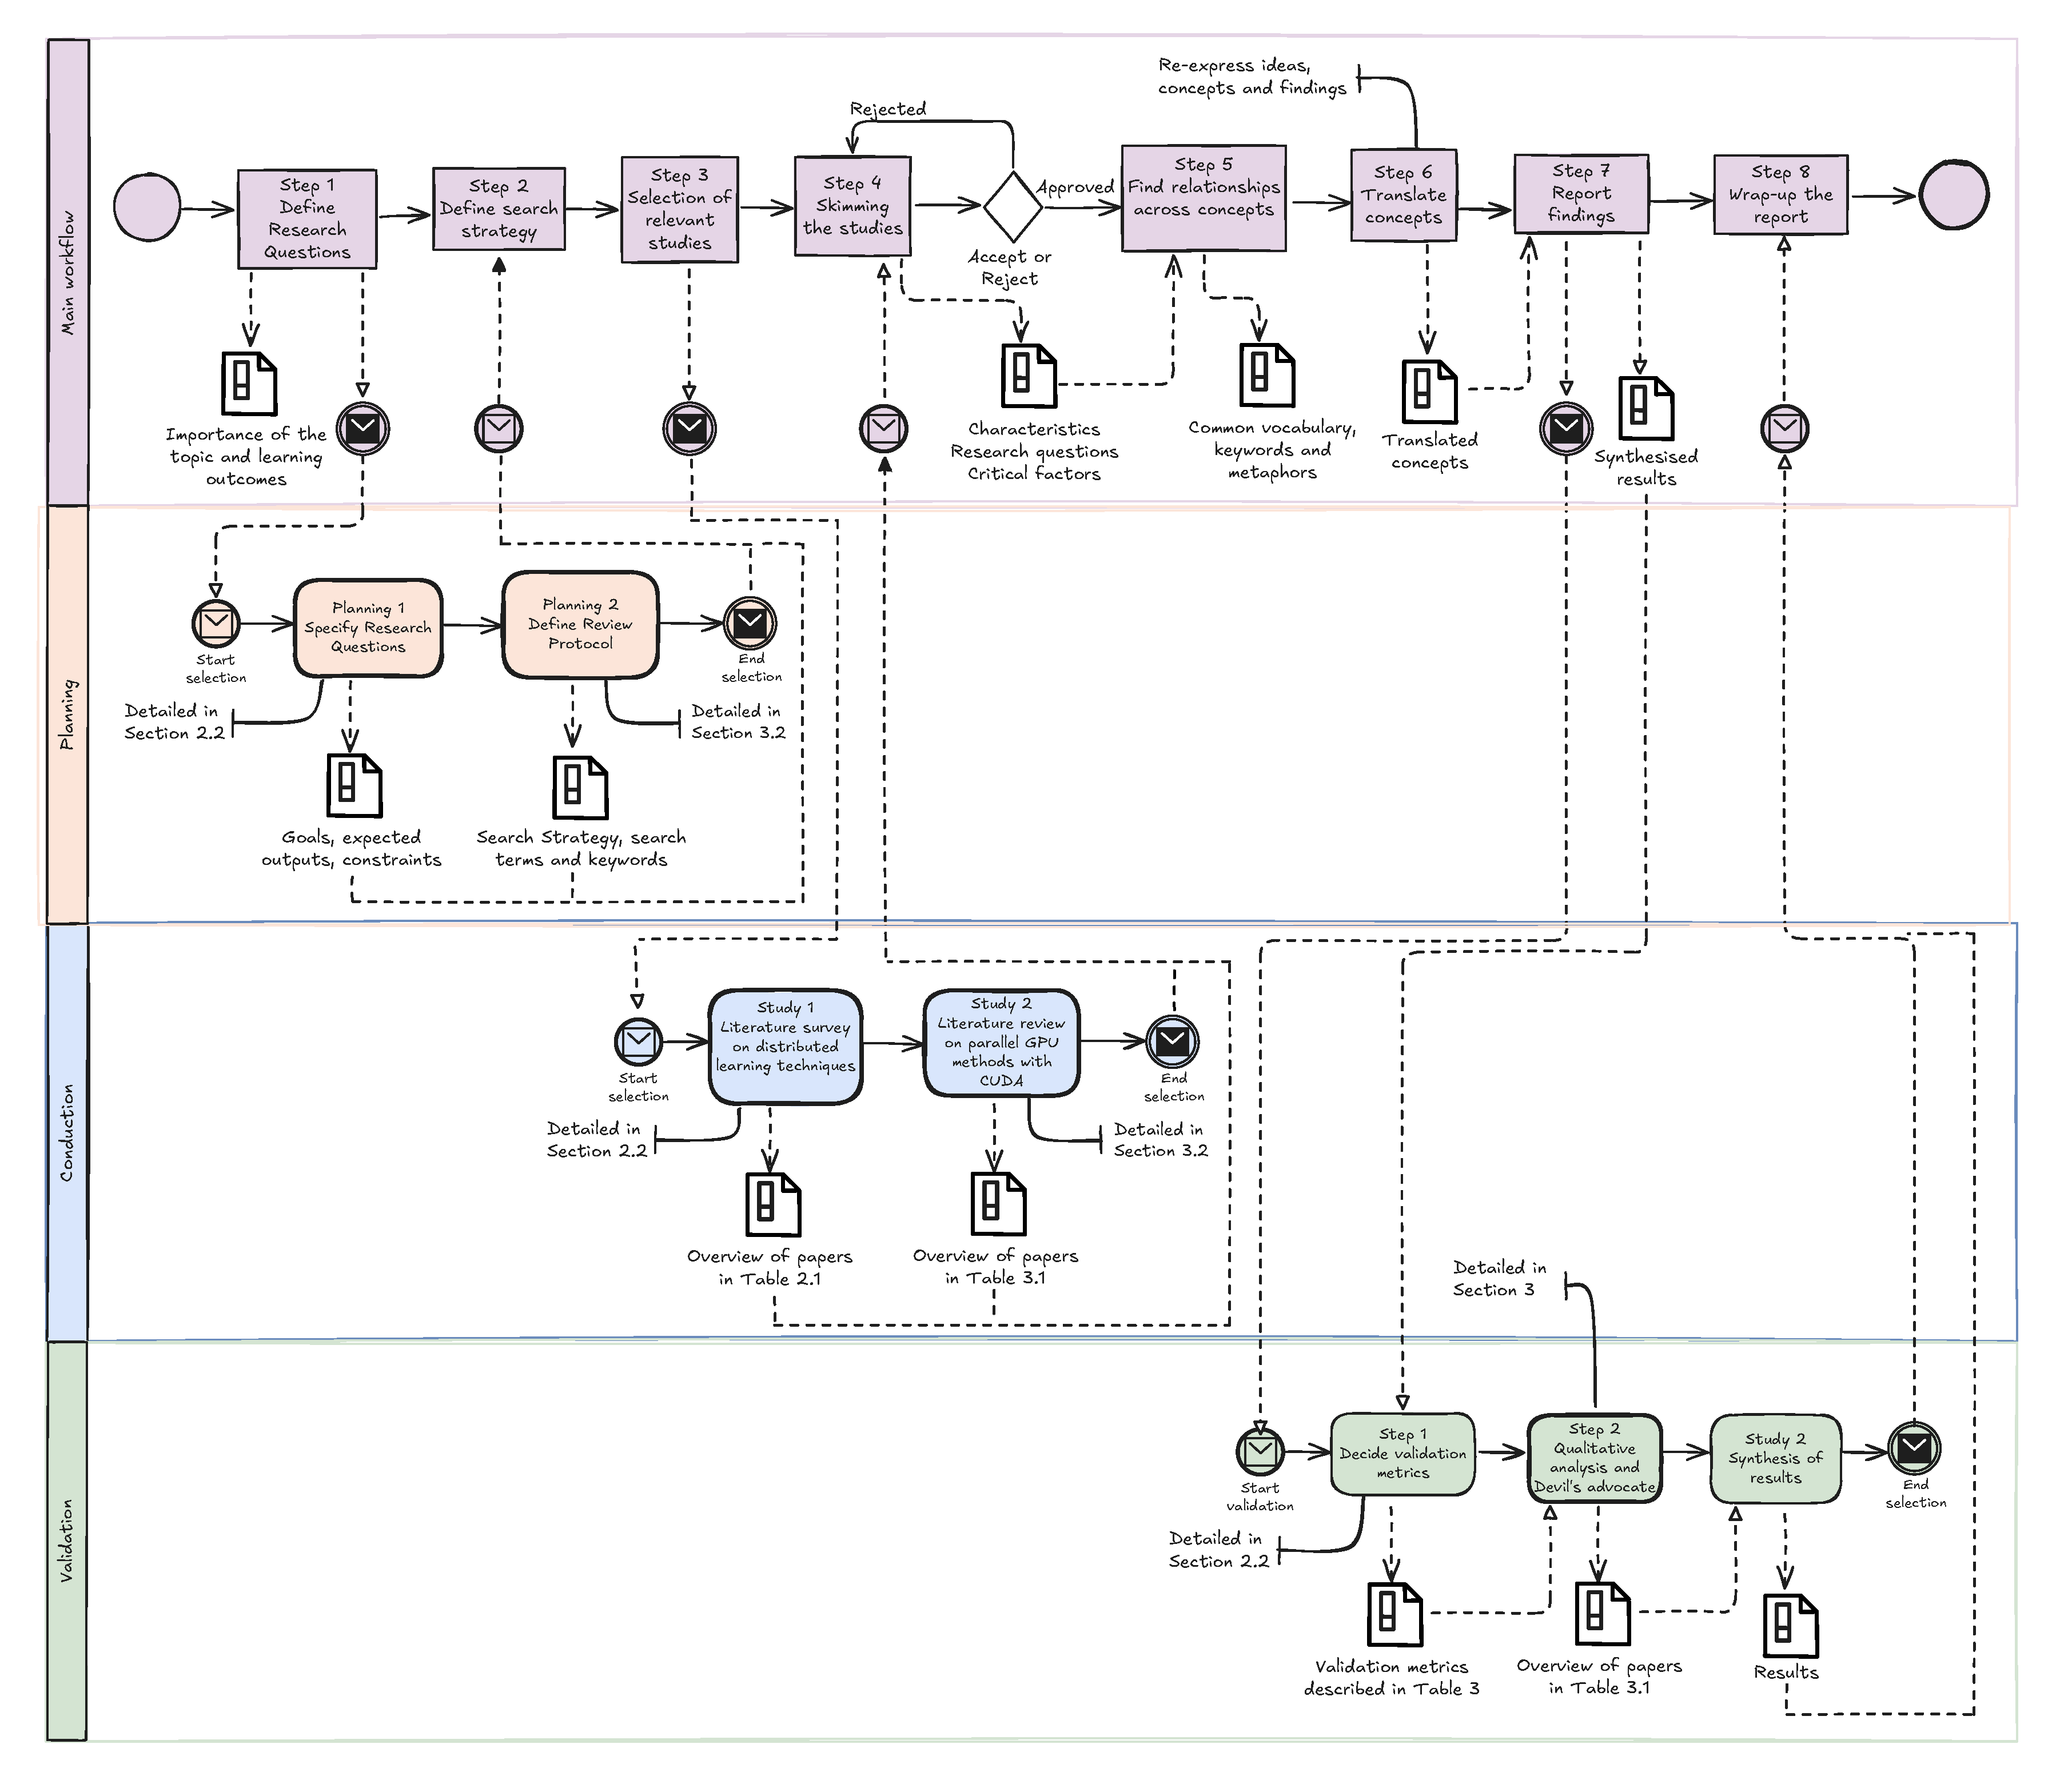
\includegraphics[width=\linewidth]{figures/workflow2}
	\caption{Systematic review workflow showing the main steps, documentation artifacts, and validation processes.
		The workflow is divided into three main phases: main workflow (top), studies selection (middle), and
		validation (bottom). Dashed lines indicate documentation and communication flows. Adapted from \cite{dos_santos_sustainable_2024}.}
	\label{fig:workflow}
\end{figure*}

\section{Related Work}
\label{sec:related_work}

\TODO{Reference the related work on survying the present methods both in DDL and CUDA}

For documenting the review process, this study follows primarily the guidelines laid out in
\cite{keele_systematic_2007}, however advice for conducting the review is synthesized from a wider
range of related articles
\cite{brereton_lessons_2007-1,kitchenham_procedures_nodate,budgen_reporting_2018,dos_santos_sustainable_2024}.

\textbf{Limitations of existing work.}
Our study differs from previous surveys in a few different aspects. First, concerning the DNN part,
related work focuses on techniques and algorithms for training models across multiple machines
\cite{dehghani_distributed_2023, chahal_hitchhikers_2018, berloco_systematic_2022}, where themes
such as data and model parallelization techniques and communication protocols are explored. As a
result, existing literature tackles architectural patterns and design choices, none focusing
explicitly on providing a broad review of the available frameworks. Secondly, although existing
repositories do provide examples on how to use the CUDA library
\cite{noauthor_nvidiacuda-samples_2025}, as well as DDP
\cite{noauthor_examplesdistributedddpreadmemd_nodate}, none provide end-to-end implementations that
would allow the community to build upon. This study aims to answer both of these concerns.

Another relevant article which aims to provide an overview of massive parallel frameworks available
for deep learning is \cite{nguyen_machine_2019}. It describes specialized tools for hardware
accelerators (GPUs, FPGAs, TPUs), however does not focus on auxiliary libraries for linear algebra,
numerical computing and GPU communication, gap which this study aims to fill.

Below are summarized some of the key concepts that the rest of this review builds upon:

\begin{itemize}
	\item \textbf{Data Parallelism:}
	      The dataset is divided across multiple nodes, with each node training a complete copy of the
	      model on its portion of data. Gradients from all nodes are then combined to update the model parameters.
	      This approach can be implemented either synchronously (all nodes wait for each other) or asynchronously (nodes work independently).

	\item \textbf{Model Parallelism:}
	      The neural network model itself is divided across different nodes, with each node responsible
	      for computing a specific portion of the model architecture. This strategy is particularly useful
	      when the model is too large to fit on a single machine.

	\item \textbf{Pipeline Parallelism:}
	      The training process is divided into sequential stages, similar to an assembly line,
	      where the output of one stage becomes the input for the next. This allows different parts
	      of the model to train simultaneously while maintaining dependencies.

	\item \textbf{Hybrid Parallelism:}
	      This approach combines multiple parallelization strategies to optimize training efficiency.
	      For example, model parallelism might be used to distribute a large model across GPUs, while
	      data parallelism is applied to each model segment.
\end{itemize}

These approaches can be further enhanced through techniques such as gradient compression, mixed
precision training, and tensor fusion \cite{dehghani_distributed_2023}. The choice of specific
techniques depends on factors including model architecture, available hardware, and training
requirements. For a comprehensive review of these techniques and their implementations, readers are
referred to \cite{chahal_hitchhikers_2018}.

\section{Research method}
\label{sec:protocol}

Multiple studies emphasize that a literature survey should be both transparent and replicable
\cite{keele_systematic_2007, dos_santos_sustainable_2024-1}, as this can ensure that review bias is
minimized. This is a valid concern in general, however especially so in this survey since it is
conducted by only one person. In a broader study, bias would normally be minimized by having
multiple iterations with more than one reviewer involved. In this paper, steps have been taken to
mitigate this problem, nonetheless it is acknowledged that it is not possible to eliminate it
completely. To ensure this, the process is documented, most of the resulting artifacts being
available in the text as well as in the Appendix.

% TODO these are all good but was hoping to minimize the number of citations
% TODO \cite{keele_systematic_2007,brereton_lessons_2007-1,budgen_reporting_2018, dos_santos_sustainable_2024-1},

% Now detail Step 1 content
The process workflow is shown in Figure \ref{fig:workflow} where the key phases are annotated as
follows: Getting Started (M.1, M.2), Planning the Review (M.3, M.4), Conducting the Review (M.5,
M.6), and Reporting the Review (M.7, M.8). M.2 calls an auxiliary process composed of S.1 and S.2
to select the appropriate studies.

\subsection{M.1 -- The need for a survey}
\label{sec:need_for_survey}

\textbf{Importance of the topic.}
Distributed techniques are important in neural networks because they allow models with billions of
parameters to perform a large number of computations in a reasonable amount of time. One of the
pioneering papers in machine learning that made use of GPUs to train neural networks in parallel
(AlexNet \cite{krizhevsky_imagenet_2012}), mentioned that the network took "between five and six days to
train on two GTX 580 3GB GPUs", suggesting that the training time would have taken much longer on a
CPU.

One key property of distributing neural network architectures to a larger number of parameters, is
that one can achieve better generalization and lower error rates even when training on smaller
datasets \cite{kaplan_scaling_2020}. This has applications in many domains, among which natural
language processing, computer vision and speech recognition \cite{noauthor_papers_nodate}.

\textbf{Learning outcomes.}
As a result of conducting the survey I expect the following learning outcomes: generally get accustomed
with the frameworks that enable distributed training of neural networks and gain practical experience
conducting experiments with CUDA and Pytorch DDP.

\subsection{M.2 -- Getting started}
\label{sec:research_questions}
The main goal is to analyze parallelization frameworks in DNNs and GPU programming. This entails two distinct
constraints: (i) consider only frameworks that introduce GPU programming and DNN frameworks and (ii) include
only primary studies.

\subsection{M.3 -- Selection of Relevant Studies}
This step identified and selected studies from both areas (GPU programming in S.1 and DNN
frameworks). I collected studies of the state of the art of both GPU programming (in Step S.1) and
DNN frameworks (in Step S.2).

\subsubsection{S.1 -- Literature Survey on DNN libraries}
\paragraph{S.1.1 -- Problem definition.}
In order to identify relevant studies, I conducted a secondary study\footnote{A secondary study
	synthesizes primary papers to provide a comprehensive overview. This contrasts with tertiary
	studies which analyze secondary studies.}. This decision was made in the problem definition step
(S.1.1 in Figure \ref{fig:workflow-study-cuda}). To ensure a methodical approach, this section
defines a research protocol which formally defines the key attributes of the search process. This
basically entails expanding on the research questions and search strategy.

\begin{figure*}[th]
	\centering
	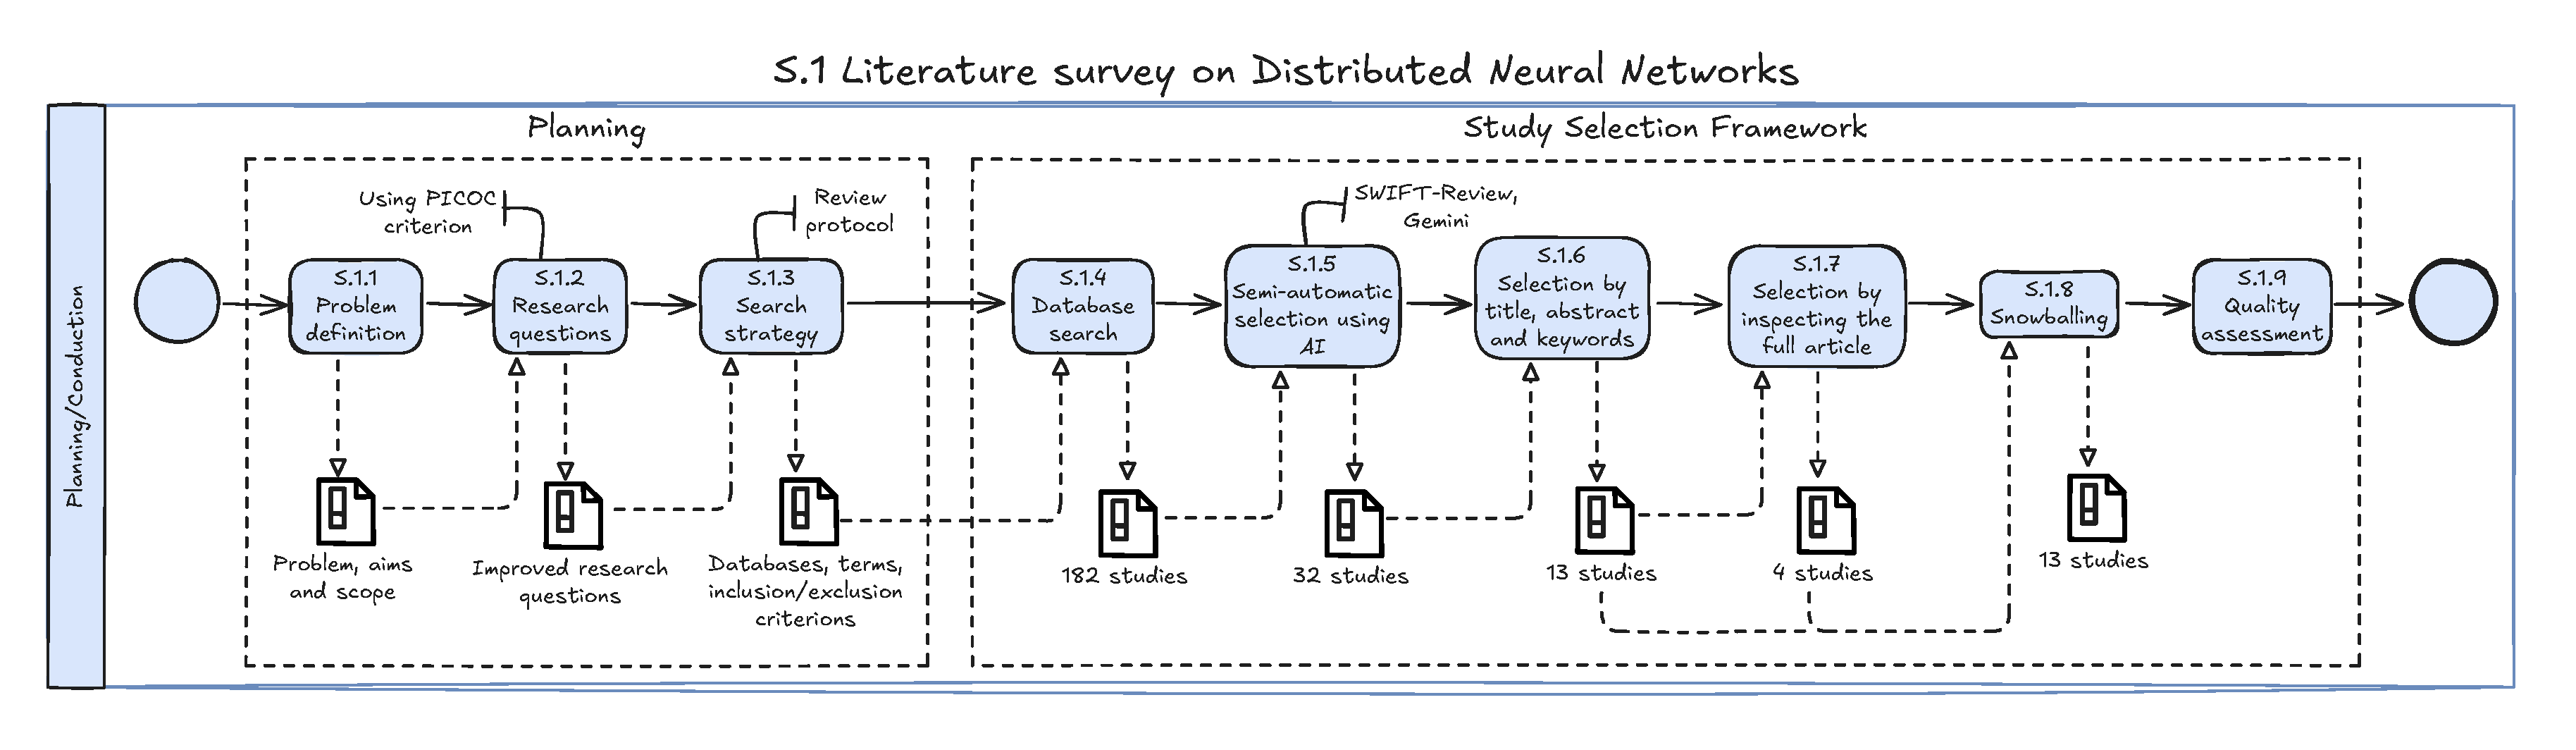
\includegraphics[width=\linewidth]{figures/survey-dnn.pdf}
	\caption{The diagram suggests the key steps for finding papers related to the CUDA programming survey. The phases
		include planning the review (aims, research questions, search strategy) and conducting the review (study selection phase). The research questions
		were transformed according to the PICOC (Population, Intervention, Comparison, Outcome, Context) criterion suggested by \cite{keele_systematic_2007}.}.
	\label{fig:workflow-study-cuda}
\end{figure*}

\paragraph{S.1.2 -- Research questions.}
After an initial literature review, the research questions (RQ) defined in Section
\ref{sec:initial_research_questions} are refined using the guidelines defined in
\cite{kitchenham_evidence-based_2015} and \cite{keele_systematic_2007}. Specifically, the PICOC
(Population, Intervention, Comparison, Outcome, Context) criterion is used to transform the
questions into a format that ensures them to be specific, measurable and well-defined. The
questions below are ordered based on their priority in the survey:

% TODO: remove this
% \begin{itemize}
% 	\item \textbf{RQ\textsubscript{1}} What are the most common frameworks currently available for 
% 		  GPU programming with CUDA, and how do their usability compare?
% 		  % NOTE implementing distributed deep learning, and how does their usability compare?
% 	      % NOTE \cite{berloco_systematic_2022, ben-nun_demystifying_2020, langer_distributed_2020}?
% 	      % NOTE \item How do parameter update strategies impact distributed deep learning systems (e.g., Parameter Server and decentralised approaches) \cite{ben-nun_demystifying_2020,berloco_systematic_2022,langer_distributed_2020}?
% 	\item How is stochastic gradient descent (SGD) computed in distributed environments
% 	      \cite{berloco_systematic_2022,ben-nun_demystifying_2020,langer_distributed_2020,verbraeken_survey_2021}? % NOTE and what are the associated challenges 
% 	\item What are the key frameworks currently available for implementing DDL, and how do their features 
% 	      compare \cite{berloco_systematic_2022}?
%  	\item In what ways are the techniques used in DDL also useful in GPU parallelization?
% \end{itemize}

% TODO: \TODO{RQ1: ease of learning, ease of use and documentation compare?}
\label{sec:research_questions_refined}
\begin{itemize}
	\item \textbf{RQ\textsubscript{1}:} In the field of Deep Learning, what are the most commonly cited
	      frameworks for distributed training of neural networks across clusters, and how do their respective communities vary in size? \\
	      \textit{Rationale:} By identifying the most common frameworks, we can trace the years in which they were published
	      and form a unified timeline of the evolution of the field. Here key motivating factors influence resulting communities.

	      % NOTE Razvan I am conducting a literature review in the field of deep learning, specifically focusing on distributed training of 
	      % NOTE neural networks across clusters. I need to identify the most commonly cited frameworks used for this purpose.
	\item \textbf{RQ\textsubscript{2}:} What practical applications of these technologies have been reported in the literature
	      and which are their limitations? \\
	      \textit{Rationale:} This can yield hands-on experience on the topic which is helpful for practical applications.

	\item \textbf{RQ\textsubscript{3}:} What are the overlaps in data/model optimization strategies used in DDL and GPU parallelization? \\
	      \textit{Rationale:} By identifying the overlaps, this can lead to a more comprehensive understanding of the field.
\end{itemize}

\tikzstyle{my-box}=[
    rectangle,
    draw=hidden-black,
    rounded corners,
    text opacity=1,
    minimum height=1.5em,
    minimum width=5em,
    inner sep=2pt,
    align=center,
    fill opacity=.5,
    % line width=0.8pt,
]
\tikzstyle{leaf}=[
    my-box, 
    minimum height=1.5em,
    % fill=hidden-orange!60, 
    fill=hidden-blue!90, 
    text=black,
    align=left,
    font=\normalsize,
    % font=\scriptsize,
    inner xsep=2pt,
    inner ysep=4pt,
    % line width=0.8pt,
]
\begin{figure*}[th!]
    \vspace{-2mm}
    \centering
    \resizebox{\textwidth}{!}{
        \begin{forest}
            forked edges,
            for tree={
                grow=east,
                reversed=true,
                anchor=base west,
                parent anchor=east,
                child anchor=west,
                base=left,
                font=\large,
                rectangle,
                draw=hidden-black,
                rounded corners,
                align=left,
                minimum width=4em,
                edge+={darkgray, line width=1pt},
                s sep=3pt,
                inner xsep=2pt,
                inner ysep=3pt,
                line width=0.8pt,
                ver/.style={rotate=90, child anchor=north, parent anchor=south, anchor=center},
            },
            where level=1{text width=10.2em,font=\normalsize,}{},
            where level=2{text width=8.5em,font=\normalsize,}{},
            where level=3{text width=10.5em,font=\normalsize,}{},
            where level=4{text width=12em,font=\normalsize,}{},
            [
                Deep Learning, ver
                [
                    GPU Programming (\S \ref{sec:task})
                    [
                        Core Libraries
                        [
                            Linear Algebra
                            [
                                \eg cuBLAS (NVIDIA)~\cite{noauthor_cublas_nodate}{,}
                                rocBLAS (AMD)~\cite{noauthor_rocmrocblas_2025}{,}
                                oneMKL (Intel)~\cite{noauthor_uxlfoundationonemath_2025}
                                , leaf, text width=32em
                            ]
                        ]
                        [
                            Deep Learning Primitives
                            [
                                \eg cuDNN (NVIDIA)~\cite{chetlur_cudnn_2014}{,}
                                MIOpen (AMD)~\cite{noauthor_rocmmiopen_2025}{,}
                                oneDNN (Intel)~\cite{onednn_contributors_oneapi_2025}
                                , leaf, text width=32em
                            ]
                        ]
                        [
                            Communication
                            [
                                \eg NCCL (NVIDIA)~\cite{noauthor_nvidianccl_2025}{,}
                                RCCL (AMD)~\cite{noauthor_rocmrccl_2025}{,}
                                oneCCL (Intel)~\cite{noauthor_uxlfoundationoneccl_2025}
                                , leaf, text width=32em
                            ]
                        ]
                    ]
                    [
                        Programming \\ Frameworks
                        [
                            Cross-Platform APIs
                            [
                                \eg OpenCL~\cite{noauthor_khronosgroupopencl-sdk_2025}{,}
                                SYCL~\cite{noauthor_khronosgroupsycl-docs_2025}{,}
                                Kokkos~\cite{trott_kokkos_2022}
                                , leaf, text width=32em
                            ]
                        ]
                        [
                            Vendor-Specific
                            [
                                \eg HIP~\cite{noauthor_rocmhip_2025}{,}
                                CUTLASS~\cite{thakkar_cutlass_2023}
                                , leaf, text width=32em
                            ]
                        ]
                    ]
                    [
                        Language Bindings
                        [
                            Julia Packages
                            [
                                \eg CUDA.jl~\cite{noauthor_juliagpucudajl_2025}{,}
                                AMDGPU.jl~\cite{noauthor_juliagpuamdgpujl_2025}{,}
                                oneAPI.jl~\cite{besard_oneapijl_2022}
                                , leaf, text width=32em
                            ]
                        ]
                        [
                            Python Packages 
                            [
                                \eg CuPy~\cite{okuta_cupy_2017}{,}
                                Numba~\cite{noauthor_numbanumba_2025}
                                , leaf, text width=32em
                            ]
                        ]
                    ]
                    [
                        Learning Resources
                        [
                            Official Tutorials
                            [
                                \eg NVIDIA-Samples~\cite{noauthor_nvidiacuda-samples_2025}{,}
                                AMD-Lab-Notes~\cite{noauthor_amdamd-lab-notes_2025}{,}
                                Intel-Compute~\cite{noauthor_intelcompute-samples_2025}
                                , leaf, text width=32em
                            ]
                        ]
                        Learning Resources
                        [
                            Literature Reviews
                            [
                                \eg Large Scale Deep Learning~\cite{nguyen_machine_2019}{,}
                                , leaf, text width=32em
                            ]
                        ]
                    ]
                ]
                [
                    Distributed Deep \\ Learning (\S \ref{sec:task})
                    [
                        Cloud Solutions
                        [
                            Cloud Platforms
                            [
                                \eg SageMaker~\cite{noauthor_amazon_nodate}{,}
                                BytePS~\cite{jiang_unified_nodate}{,}
                                AzureML~\cite{sdgilley_azure_nodate}{,}
                                Vertex AI~\cite{noauthor_vertex_nodate}
                                , leaf, text width=32em
                            ]
                        ]
                    ]
                    [
                        Framework-Specific
                        [
                            Core Frameworks
                            [
                                \eg PyTorch~\cite{li_pytorch_2020}{,}
                                TensorFlow~\cite{abadi_tensorflow_2016}{,}
                                MXNet~\cite{chen_mxnet_2015}{,}
                                JAX~\cite{frostig_compiling_nodate}
                                , leaf, text width=32em
                            ]
                        ]
                        [
                            Extensions
                            [
                                \eg Transformers~\cite{wolf_huggingfaces_2020}{,}
                                Lightning~\cite{noauthor_overview_nodate}
                                , leaf, text width=32em
                            ]
                        ]
                    ]
                    [
                        General-Purpose
                        [
                            Universal Frameworks
                            [
                                \eg Colossal-AI~\cite{li_colossal-ai_2023}{,}
                                Ray~\cite{moritz_ray_2018}{,}
                                Horovod~\cite{sergeev_horovod_2018}
                                , leaf, text width=32em
                            ]
                        ]
                    ]
                    [
                        Specialized Tools
                        [
                            Large Model Training
                            [
                                \eg Megatron-LM~\cite{shoeybi_megatron-lm_2020}{,}
                                GPipe~\cite{huang_gpipe_2019}{,}
                                DeepSpeed~\cite{rasley_deepspeed_2020}{,}
                                FairScale~\cite{noauthor_fairscale_nodate}
                                , leaf, text width=32em
                            ]
                        ]
                        [
                            Research
                            [
                                \eg GShard~\cite{lepikhin_gshard_2020}
                                , leaf, text width=32em
                            ]
                        ]
                    ]
                    [
                        [
                            Distributed
                            [
                                \eg Pylearn2~\cite{Goodfellow.EtAl_2013}{,} Torch7~\cite{Collobert.EtAl_}{,} Caffe~\cite{Jia.EtAl_2014a}{,} Cuda-Convnet~\cite{krizhevsky_imagenet_2012}
                                , leaf, text width=32em
                            ]
                        ]
                    ]
                    [
                        Learning Resources
                        [
                            Official Tutorials
                            [
                                \eg Pytorch DDP~\cite{noauthor_examplesdistributedddpreadmemd_nodate}
                                , leaf, text width=32em
                            ]
                        ]
                        Learning Resources
                        [
                            Literature Reviews
                            [
                                \eg Distributed Deep Learning Surveys~\cite{dehghani_distributed_2023}{,}
                                \cite{chahal_hitchhikers_2018}{,}
                                \cite{berloco_systematic_2022}
                                , leaf, text width=32em
                            ]
                        ]
                    ]
                ]
            ]
        \end{forest}
    }
    \vspace{-4mm}
    \caption{Taxonomy of deep learning for mathematical reasoning. The associated tasks are elaborated in \S \ref{sec:task}, with a comprehensive dataset list found in \S \ref{sec:dataset}. Deep learning methods are further discussed in \S \ref{sec:network}, \S \ref{sec:pretrain}, and \S \ref{sec:icl}.}
    \label{fig:taxonomy}
    \vspace{-3mm}
\end{figure*}
The questions play a key role in guiding the search strategy, data extraction process and results
synthesis phase.

\paragraph{S.1.3 -- Search Strategy.}
The search strategy represents represents a systematic approach for identifying relevant studies
that adequately answer the research questions.

\textbf{Databases.}
The process involves a manual search of three citation databases --
\href{https://www.scopus.com/}{Scopus}, \href{https://www.semanticscholar.org/}{Semantic Scholar}
and \href{https://arxiv.org/}{arXiv}\footnote{Other relevant databases that could have been used
	include: \href{https://ieeexplore.ieee.org/}{IEEE Xplore}, \href{https://dl.acm.org/}{ACM Digital
		Library} and \href{https://www.sciencedirect.com/}{Science Direct}.} -- that include conference
proceedings and journal papers, considering three metadata fields (title, abstract, and keywords).

\textbf{Inclusion/Exclusion Criteria.}
There were defined three inclusion criteria (IC) and three exclusion criteria (EC). In particular, I
decided to select only primary studies, however secondary studies were mentioned in Section
\ref{sec:related_work}. The identification of secondary studies was useful since the selected
studies synthesize evidence and can make it possible to access primary studies:

\begin{itemize}
	\item \textbf{IC\textsubscript{1}}: Study is a primary study.
	\item \textbf{IC\textsubscript{2}}: Study addresses distributed frameworks in DL.
	\item \textbf{IC\textsubscript{3}}: Study introduces a library or a framework. \\
	\item \textbf{EC\textsubscript{1}}: Study does not discuss implementation details.
	\item \textbf{EC\textsubscript{2}}: Study is not a primary study.
	\item \textbf{EC\textsubscript{3}}: Study is not written in English.
\end{itemize}

\textbf{Search terms.}
In Step S.1.3, I inquired about the literature using the following search string:
\begin{quote}
	\textit{( "machine learning" OR "deep learning" )
		AND
		( "Data parallelism" OR "model parallelism")
		AND
		( "framework" OR "implementation" )}
\end{quote}

The details and justification to define this search string can be found in the supplementary
material in Section \ref{sec:search_strategy}. \TODO{...}

\paragraph{Publication year criteria.}
For the DDL task, papers were considered between $\yearstartddl$-$\yearendddl$. The start year
($\yearstartddl$) was chosen as at this point there was a shift towards resource conservation,
which resulted in a focus on concurrency within mini-batches \cite{ben-nun_demystifying_2020}. This
is the year by which the effectiveness of deep learning algorithms was more widely recognized and
more research was published that focused on scalability.

\paragraph{S1.4 - S1.5 -- Semi-Automatic selection.}
After an initial database search (Step S1.4), 182 studies were retrieved. Subsequently, as part of
S.1.5, two methods were applied for reducing the number of studies to a more manageable set. Below,
I describe each approach, including my evaluation regarding their effectiveness.

\textbf{Swift-Review.}
As suggest in \cite{bolanos_artificial_2024},
I applied Swift-Review \cite{Howard2016SWIFTReviewAT}, a machine learning classifier to filter out
irrelevant studies (Step S.1.5). The technique is semi-automatic
with a focus on screening and extraction of relevant information. Prior to initiating the classification,
I had to manually identify 10 positive and 10 negative examples. These
acted as input seed samples for the classifier, which helped pinpoint other useful material. Then
the classifier identified other relevant papers by screening the title, abstract and keywords of
each study. All papers with a confidence score above 0.5 are selected.

\textbf{Classification using Gemini.}
The downside of the previous approach is that it still involves a lot of work to manually identify key
studies. To address this, \cite{bolanos_artificial_2024} suggests many emerging tools that use Large Language Models (LLMs)
to automatically classify relevant material. However, in my experience, none are particularly effective
at handling a large corpus of text due to the context window being relatively small. As a result, I decided
to use Gemini \cite{team_gemini_2024} to classify the studies, which is a particularly strong choice due to its massive
context window (over 2M tokens). The drawback is that Gemini does not provide citations when using the web interface
\cite{noauthor_gemini_nodate}. However, NotebookLM \cite{notebooklm_google_2024} solves the issue by providing references
to portions of the text that are relevant to the query. My approach involved downloading the search results in textual format from the
search engines and then leveraging NotebookLM to classify the studies by utilizing the research questions
defined in Section \ref{sec:research_questions} as a prompt. This was an iterative process that involved
reading the abstracts and keywords of each study to ascertain about the reliability of each response. It is not a perfect process,
however building iteratively over the results and blending together different phases of the review process
(as we shall see in Section \ref{sec:reading-studies}), gives a good baseline for iterative improvement.

\textbf{Results.}
After investigating the results of both approaches, I found that the NotebookLM approach was more
effective at identifying key studies. This is likely due to Gemini being a more powerful
model than the classifier used by Swift-Review. The number of selected studies was 32.
  
\begin{table*}[th!]
	\centering
	\caption{A list of papers on Distributed Neural Networks}
	\label{tab:dnn_papers}
	\begin{tabular}{llp{8.4cm}lllc}
		\hline
		\small \textbf{\#} & \small \textbf{Ref.}                    & \small \textbf{Title}                                                                                                               & \small \textbf{Type} & \small \textbf{Year} & \small \textbf{Citations} & \small \textbf{Stars}                                                \\[1ex]
		\hline
		\small DNN1        & \small \cite{abadi_tensorflow_2016}     & \small TensorFlow: Large-Scale Machine Learning on Heterogeneous Distributed Systems                                                & \small Data          & \small 2016          & \small 9998               & \small 187k \cite{abadi_tensorflow_2015}                             \\[1ex]
		\small DNN2        & \small \cite{chen_mxnet_2015}           & \small MXNet: A Flexible and Efficient Machine Learning Library for Heterogeneous Distributed Systems                               & \small Hybrid        & \small 2015          & \small 2214               & \small 20.8k \cite{noauthor_apachemxnet_2025}                        \\[1ex]
		\small DNN3        & \small \cite{huang_gpipe_2019}          & \small GPipe: Efficient Training of Giant Neural Networks using Pipeline Parallelism                                                & \small Pipeline      & \small 2018          & \small 1446               & \small 2.8k \cite{noauthor_tensorflowlingvo_2025}                    \\[1ex]
		\small DNN4        & \small \cite{jiang_unified_nodate}      & \small BytePS: A Unified Architecture for Accelerating Distributed DNN Training in Heterogeneous GPU/CPU Clusters                   & \small Data          & \small 2020          & \small 338                & \small 3.7k \cite{noauthor_bytedancebyteps_2025}                     \\[1ex]
		\small DNN5        & \small \cite{lepikhin_gshard_2020}      & \small GShard: Scaling Giant Models with Conditional Computation and Automatic Sharding                                             & \small Model         & \small 2020          & \small 931                & \small 2.8k \cite{noauthor_tensorflowlingvo_2025}                    \\[1ex]
		\small DNN6        & \small \cite{li_pytorch_2020}           & \small PyTorch Distributed: Experiences on Accelerating Data Parallel Training                                                      & \small Hybrid        & \small 2020          & \small 175                & \small 86.1k \cite{noauthor_pytorchpytorch_nodate}                   \\[1ex]
		\small DNN7        & \small \cite{li_colossal-ai_2023}       & \small Colossal AI: A Unified Deep Learning System for Large-Scale Parallel Training                                                & \small Hybrid        & \small 2023          & \small 118                & \small 39k \cite{noauthor_hpcaitechcolossalai_2025}                  \\[1ex]
		\small DNN8        & \small \cite{moritz_ray_2018}           & \small Ray: A distributed Framework for Emerging AI Applications                                                                    & \small Hybrid        & \small 2018          & \small 1108               & \small 35k \cite{noauthor_ray-projectray_2025}                       \\[1ex]
		\small DNN9        & \small \cite{rasley_deepspeed_2020}     & \small DeepSpeed: System Optimizations Enable Training Deep Learning Models with Over 100 Billion Parameters                        & \small Hybrid        & \small 2020          & \small 1059               & \small 36.3k \cite{noauthor_microsoftdeepspeed_2025}                 \\[1ex]
		\small DNN10       & \small \cite{sergeev_horovod_2018}      & \small Horovod: fast and easy distributed deep learning in TensorFlow                                                               & \small Data          & \small 2018          & \small 1152               & \small 14.3k \cite{noauthor_horovodhorovod_2025}                     \\[1ex]
		\small DNN11       & \small \cite{shoeybi_megatron-lm_2020}  & \small Megatron-LM: Training Multi-Billion Parameter Models for Natural Language Processing                                         & \small Hybrid        & \small 2020          & \small 1578               & \small 11.2k \cite{noauthor_nvidiamegatron-lm_2025}                  \\[1ex]
		\small DNN12       & \small \cite{wolf_huggingfaces_2020}    & \small HuggingFace's Transformers: State-of-the-art Natural Language Processing                                                     & \small Data          & \small 2020          & \small 1444               & \small 8.2k \cite{noauthor_huggingfaceaccelerate_2025}               \\[1ex]
		\small DNN13       & \small \cite{noauthor_overview_nodate}  & \small Pytorch Lightning: The lightweight PyTorch wrapper for high-performance AI research. Scale your models, not the boilerplate. & \small Data          & \small 2019          & \small N/A                & \small 28.8k \cite{falcon_pytorch_2019}                              \\[1ex]
		\small DNN14       & \small \cite{noauthor_fairscale_nodate} & \small FairScale:  A general purpose modular PyTorch library for high performance and large scale training                          & \small Hybrid        & \small 2021          & \small N/A                & \small 3.2k \cite{FairScale2021}                                     \\[1ex]
		\small DNN15       & \small \cite{noauthor_amazon_nodate}    & \small Amazon SageMaker Platform                                                                                                    & \small Data          & \small 2017          & \small N/A                & \small 10.3k \cite{noauthor_awsamazon-sagemaker-examples_2025}       \\[1ex]
		\small DNN16       & \small \cite{sdgilley_azure_nodate}     & \small Microsoft AzureML Platform                                                                                                   & \small Data          & \small 2021          & \small N/A                & \small 1.8k \cite{noauthor_azureazureml-examples_2025}               \\[1ex]
		\small DNN17       & \small \cite{noauthor_vertex_nodate}    & \small Google Vertex AI Platform                                                                                                    & \small Data          & \small 2021          & \small N/A                & \small 178 \cite{noauthor_googlecloudplatformvertex-ai-samples_2025} \\[1ex]
		\small DNN18       & \small \cite{frostig_compiling_nodate}  & \small Jax: Compiling machine learning programs via high-level tracing                                                              & \small Hybrid        & \small 2018          & \small N/A                & \small 31k \cite{noauthor_jax-mljax_2025}                            \\[1ex]
		\hline
	\end{tabular}
\end{table*}


\paragraph{S.1.6 - S.1.8 -- Manual selection.}
In Step S.1.6, a manual inspection over the the title, abstract and keywords was made. This
resulted in a total of 13 studies that appeared to be relevant. After checking their full text,
this number was reduced to 4. I performed backward snowballing \cite{jalali_systematic_2012} by
revisiting the references of the 4 studies, as well as checking available preprint articles and
identified other 8 studies (Step 1.8). Hence, a total of 12 studies (4 + 8) were selected. A
subsequent 5 frameworks were found with no accompanying papers by reviewing the references. All 17
libraries are listed in Table \ref{tab:dnn_papers}.

\begin{table}[h!]
	\centering
	\caption{The Search Engines Used in this Survey}
	\label{tab:databases}
	\begin{tabular}{llllr}
		\hline
		ID    & Tool             & Step  & Results & Filtered \\
		\hline
		1     & Scopus           & S.1.4 & 182     & 4        \\
		2     & Semantic Scholar & S.1.8 & --      & 8        \\
		3     & Proprietary      & S.1.8 & --      & 5        \\
		\hline
		Total &                  &       &         & 17       \\
	\end{tabular}
\end{table}

\paragraph{S.1.9 -- Quality assessment.}
To evaluate the quality of these studies (Step S.1.9), I adapted the quality appraisal instrument
suggested by \cite{zhou_map_2016}, considering 2 main aspects: report and relevance. Regarding
report, I checked whether the studies clearly tackled the problem, research questions and
inclusion/exclusion criteria defined in Steps S.1.1, S.1.2 and S.1.3 respectively. Concerning
relevance, I verified whether the studies presented relevant information to ensure their value for
practitioners and researchers. Finally, all 17 studies identified in the previous steps passed the
quality checks.

\begin{figure*}[th]
	\centering
	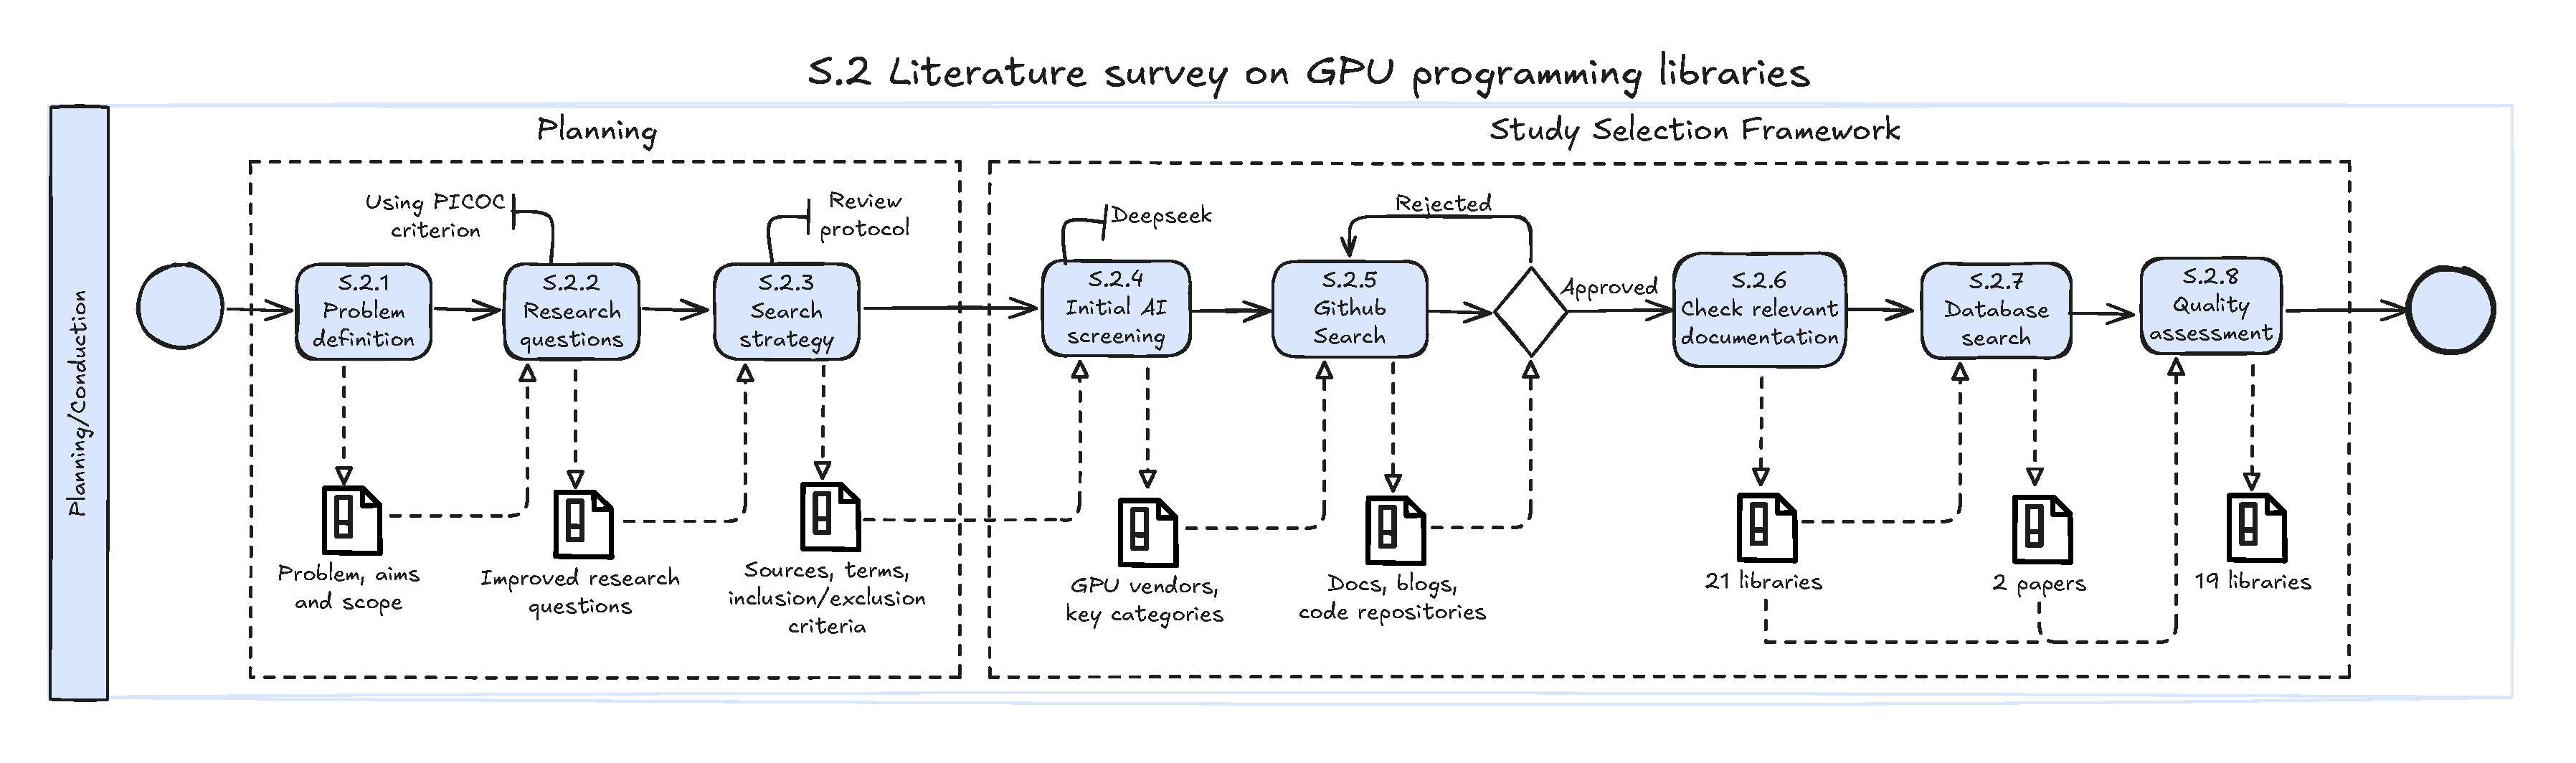
\includegraphics[width=\linewidth]{figures/survey-cuda3.pdf}
	\caption{The diagram suggests the key steps for finding papers related to the CUDA programming survey. The phases
		include planning the review (aims, research questions, search strategy) and conducting the review (study selection phase). The research questions
		were transformed according to the PICOC (Population, Intervention, Comparison, Outcome, Context) criterion suggested by \cite{keele_systematic_2007}.}.
	\label{fig:workflow-study-dnn}
\end{figure*}
\subsubsection{S.2 -- Survey on GPU programming libraries}
\label{sec:gpu-programming-libraries}
This step involved identifying popular frameworks that facilitate programming on the GPU. The
workflow that was followed is shown in Figure \ref{fig:workflow-study-cuda}.

\paragraph{S.2.1 -- Problem definition.}
It was not possible to perform a systematic review in the traditional sense due to the nature of
the available tools. The available libraries are frequently proprietary and are rarely accompanied
by academic papers. Also, the libraries are implementation-focused with documentation and tutorials
being the main source of information. As a result, I had to widen out the type of articles to
include in the review by referencing useful tutorials and key documentation pages.

\paragraph{S.2.2 -- Research Questions.}
The research questions defined in Section \ref{sec:initial_research_questions} were refined using
the PICOC criterion suggested by \cite{keele_systematic_2007}. The following question is relevant:

\begin{itemize}
	\item \textbf{RQ\textsubscript{4}:} In the field of Deep Learning, what are the most frequently cited
	      frameworks for GPU programming using CUDA, and how do their user communities differ in size? \\
	      \textit{Rationale:} By identifying the most common frameworks, we can identify which are the gaps
	      in the literature they cover and which are the most promising areas for future research.
\end{itemize}

Moreover, questions RQ\textsubscript{2} and RQ\textsubscript{3} from Section
\ref{sec:research_questions_refined} are also relevant.

\paragraph{S.2.3 -- Search strategy.}
To find relevant materials (Github repositories, documentation pages and tutorials), the following
tools were used: \href{https://github.com/search/advanced}{Advanced Github Search} and two AI
search engines: DeepSeek Search Engine \cite{noauthor_deepseek_nodate} and Perplexity AI
\cite{noauthor_perplexity_nodate}.

\textbf{Inclusion/Exclusion criteria.}
The following criteria were identified to guide the selection process:

\begin{itemize}
	\item \textbf{IC\textsubscript{1}}: The material addresses GPU programming.
	\item \textbf{IC\textsubscript{2}}: The material is official documentation/repository.
	\item \textbf{IC\textsubscript{3}}: The material is a tutorial.
	\item \textbf{IC\textsubscript{4}}: The material introduces a library or framework. \\
	\item \textbf{EC\textsubscript{1}}: The material is not a primary source.
	\item \textbf{EC\textsubscript{2}}: The material is not written in English.
\end{itemize}

\textbf{Search terms.}
The following terms were used to process the search for relevant Github repositories, which are
linked to the main GPU manufacturers:

\begin{quote}
	\textit{user:ROCm user:oneAPI-SRC user:NVIDIA}
\end{quote}

These correspond to AMD, Intel and NVIDIA official repositories in Github.

\textbf{Publication year criteria.}
The GPU programming search was restricted to papers published between
$\yearstartcuda$-$\yearendcuda$. The start year ($\yearstartcuda$) was chosen as the baseline due
to being the year when AlexNet \cite{krizhevsky_imagenet_2012} was published. This paper
revolutionized research in neural networks by allowing advanced AI models to be trained on GPUs.

\paragraph{S.2.4 - S.2.8 -- Study Selection Framework.}
\label{sec:ai-screening}
At this step, I used DeepSeek \cite{noauthor_deepseek_nodate} to identify relevant GPU programming
keywords and categories (Step S.2.4). This led to identifying \cite{noauthor_enccsgpu-programming_nodate}, which
offers an excellent introduction to the topic covering general aspects of GPU programming as well
as specific frameworks.

\begin{figure*}[htbp]
    \centering
    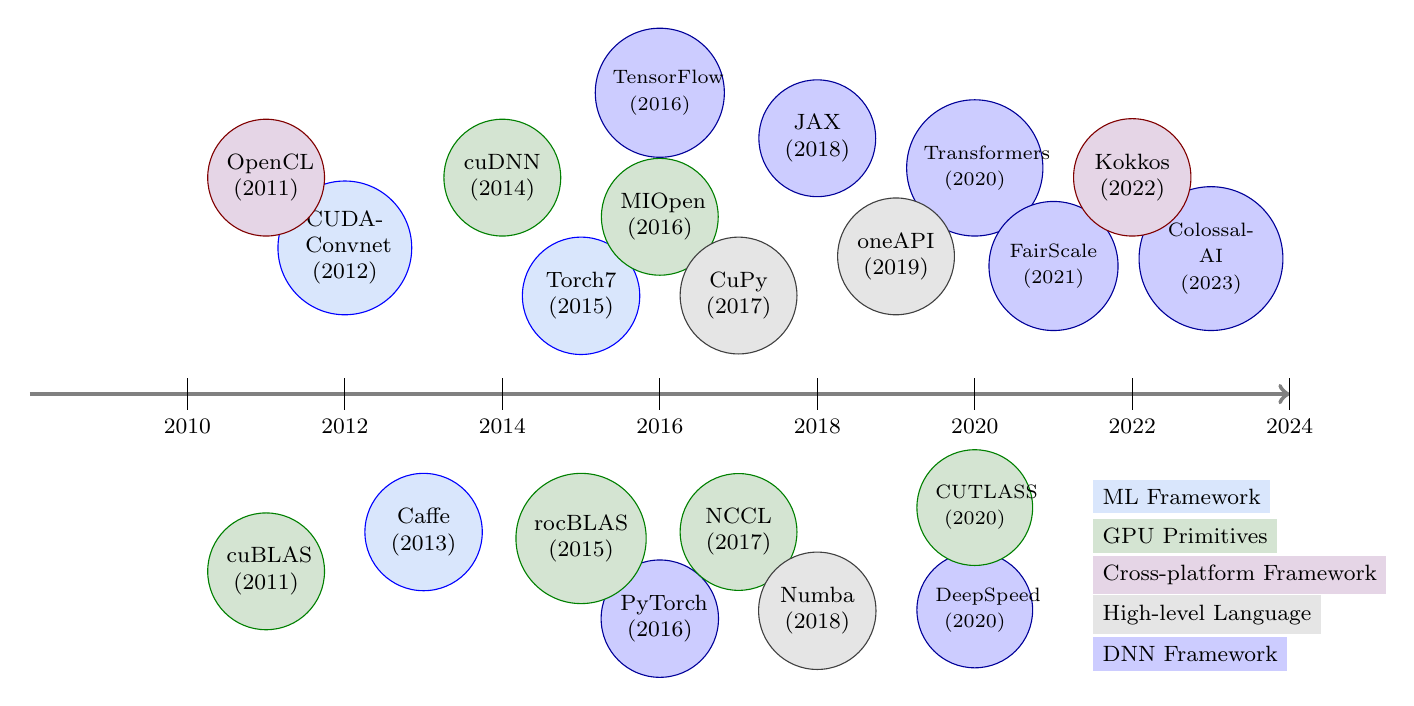
\begin{tikzpicture}[
        timeline/.style={
            ->,
            ultra thick,
            draw=gray
        },
        event/.style={
            circle,
            fill=blue!20,  % Hex: #d9e6fc
            draw=blue!60!black,
            text width=1cm,
            align=center,
            font=\footnotesize
        },
        levent/.style={
            circle,
            fill=blue!20,  % Hex: #d9e6fc
            draw=blue!60!black,
            text width=1.2cm,
            align=center,
            font=\footnotesize
        },
        llevent/.style={
            circle,
            fill=blue!20,  % Hex: #d9e6fc
            draw=blue!60!black,
            text width=1.3cm,
            align=center,
            font=\footnotesize
        },
        core/.style={
            circle,
            fill={rgb,255:red,212; green,228; blue,210},  % Hex: #d4e4d2
            draw=green!50!black,
            text width=1cm,
            align=center,
            font=\footnotesize
        },
        lcore/.style={
            circle,
            fill={rgb,255:red,212; green,228; blue,210},  % Hex: #d4e4d2
            draw=green!50!black,
            text width=1.2cm,
            align=center,
            font=\footnotesize
        },
        framework/.style={
            circle,
            fill={rgb,255:red,229; green,213; blue,230},  % Hex: #e5d5e6
            draw=red!50!black,
            text width=1cm,
            align=center,
            font=\footnotesize
        },
        language/.style={
            circle,
            fill=gray!20,
            draw=gray!50!black,
            text width=1cm,
            align=center,
            font=\footnotesize
        },
        eventg/.style={
            circle,
            fill={rgb,255:red,217; green,230; blue,252},
            draw=blue,
            text width=1cm,
            align=center,
            font=\footnotesize
        },
        leventg/.style={
            circle,
            fill=blue!20,
            draw=blue,
            text width=1.2cm,
            align=center,
            font=\footnotesize
        },
        lleventg/.style={
            circle,
            fill=blue!20,
            draw=blue,
            text width=1.3cm,
            align=center,
            font=\footnotesize
        },
        nvidia/.style={
            circle,
            fill=green!20,
            draw=green!50!black,
            text width=1cm,
            align=center,
            font=\footnotesize
        },
        amd/.style={
            circle,
            fill=red!20,
            draw=red!50!black,
            text width=1cm,
            align=center,
            font=\footnotesize
        },
        lamd/.style={
            circle,
            fill=red!20,
            draw=red!50!black,
            text width=1.2cm,
            align=center,
            font=\footnotesize
        },
        cross/.style={
            circle,
            fill=gray!20,
            draw=gray!50!black,
            text width=1cm,
            align=center,
            font=\footnotesize
        }
    ]
        % Main timeline
        \draw[timeline] (-2,0) -- (14,0);
        
        % Time markers
        \foreach \x/\year in {0/2010,2/2012,4/2014,6/2016,8/2018,10/2020,12/2022,14/2024} {
            \draw (\x,-0.2) -- (\x,0.2);
            \node[below] at (\x,-0.2) {\footnotesize \year};
        }
        
        % Original events
        \node[eventg, above] at (2,1) {CUDA-Convnet (2012)};
        \node[eventg, below] at (3,-1) {Caffe (2013)};
        \node[eventg, below] at (5,2) {Torch7 (2015)};
        

        
        % New DL framework events
        \node[levent, above] at (6,3) {{\scriptsize TensorFlow (2016)}};
        \node[event, below] at (6,-2.1) {PyTorch (2016)};
        \node[event, above] at (8,2.5) {JAX (2018)};
        \node[llevent, above] at (10,2) {{\scriptsize Transformers (2020)}};
        \node[event, below] at (10,-2) {{\scriptsize DeepSpeed (2020)}};
        \node[levent, above] at (11,0.8) {{\scriptsize FairScale (2021)}};
        \node[levent, above] at (13,0.8) {{\scriptsize Colossal-AI (2023)}};
        
        % ============== GPU ==============
        % Core technologies
        \node[core, above] at (1,-3) {cuBLAS (2011)};
        \node[core, above] at (4,2) {cuDNN (2014)};
        \node[core, above] at (7,-2.5) {NCCL (2017)};
        \node[core, below] at (10,-0.7) {{\scriptsize CUTLASS (2020)}};
        \node[lcore, below] at (5,-1) {rocBLAS (2015)};
        \node[core, below] at (6,3) {MIOpen (2016)};
        
        % Framework solutions
        \node[framework, above] at (1,2) {OpenCL (2011)};
        \node[framework, above] at (12,2) {Kokkos (2022)};
        
        % Language tools
        \node[language, below] at (7,2) {CuPy (2017)};
        \node[language, below] at (8,-2) {Numba (2018)};
        \node[language, above] at (9,1) {oneAPI (2019)};
        
        % ============== Legend ==============
        % Type color coding
        \node[draw=none, fill={rgb,255:red,217; green,230; blue,252}, right] at (11.5, -1.3) {\footnotesize ML Framework};  % Hex: #d9e6fc
        \node[draw=none, fill={rgb,255:red,212; green,228; blue,210}, right] at (11.5, -1.8) {\footnotesize GPU Primitives};  % Hex: #d4e4d2
        \node[draw=none, fill={rgb,255:red,229; green,213; blue,230}, right] at (11.5, -2.3) {\footnotesize Cross-platform Framework};  % Hex: #e5d5e6
        \node[draw=none, fill=gray!20, right] at (11.5, -2.8) {\footnotesize High-level Language};
        \node[draw=none, fill=blue!20, right] at (11.5, -3.3) {\footnotesize DNN Framework};
    \end{tikzpicture}
    \caption{Timeline of Major GPU Programming Libraries and Frameworks}
    \label{fig:timeline}
\end{figure*} 


\begin{table*}[htbp]
	\centering
	\caption{A list of libraries and frameworks for GPU programming}
	\label{tab:gpu_papers}
	\begin{tabular}{llp{8cm}lll}
		\hline
		\small \textbf{Category} & \small \textbf{ID} & \small \textbf{Library/Framework}                                                     & \small \textbf{Vendor} & \small \textbf{Type} & \small \textbf{Ref.}                                  \\
		\hline
		\multirow{5}{*}{\small NVIDIA}
		                         & \small NV1         & \small cuBLAS: GPU-accelerated BLAS library for linear algebra                        & \small NVIDIA          & \small Core          & \small \cite{noauthor_cublas_nodate}                  \\[1ex]
		                         & \small NV2         & \small cuDNN: Optimized deep neural network primitives                                & \small NVIDIA          & \small Core          & \small \cite{chetlur_cudnn_2014}                      \\[1ex]
		                         & \small NV4         & \small NCCL: Multi-GPU/multi-node communication                                       & \small NVIDIA          & \small Core          & \small \cite{noauthor_nvidianccl_2025}                \\[1ex]
		                         & \small NV5         & \small CUTLASS: Optimized C++ templates for matrix multiplication                     & \small NVIDIA          & \small Core          & \small \cite{thakkar_cutlass_2023}                    \\
		\hline
		\multirow{5}{*}{\small AMD}
		                         & \small AMD1        & \small rocBLAS: AMD's BLAS implementation                                             & \small AMD             & \small Core          & \small \cite{noauthor_rocmrocblas_2025}               \\[1ex]
		                         & \small AMD2        & \small MIOpen: Deep learning primitives                                               & \small AMD             & \small Core          & \small \cite{noauthor_rocmmiopen_2025}                \\[1ex]
		                         & \small AMD3        & \small HIP: Portable API for CUDA-like code                                           & \small Multiple        & \small Framework     & \small \cite{noauthor_rocmhip_2025}                   \\[1ex]
		                         & \small AMD4        & \small RCCL: Multi-GPU communication                                                  & \small AMD             & \small Core          & \small \cite{noauthor_rocmrccl_2025}                  \\
		\hline
		\multirow{4}{*}{\small Intel}
		                         & \small INT1        & \small oneMKL: Math Kernel Library                                                    & \small Intel           & \small Core          & \small \cite{noauthor_uxlfoundationonemath_2025}      \\[1ex]
		                         & \small INT2        & \small oneDNN: Deep learning primitives                                               & \small Intel           & \small Core          & \small \cite{onednn_contributors_oneapi_2025}         \\[1ex]
		                         & \small INT3        & \small oneCCL: Collective communication library                                       & \small Intel           & \small Core          & \small \cite{noauthor_uxlfoundationoneccl_2025}       \\
		\hline
		\multirow{4}{*}{\small Cross-Platform}
		                         & \small CP1         & \small OpenCL: Open standard for heterogeneous computing                              & \small Multiple        & \small Framework     & \small \cite{noauthor_khronosgroupopencl-sdk_2025}    \\[1ex]
		                         & \small CP2         & \small SYCL: C++-based multi-device programming                                       & \small Multiple        & \small Framework     & \small \cite{noauthor_khronosgroupsycl-docs_2025}     \\[1ex]
		                         & \small CP3         & \small Kokkos: Performance-portable C++ framework                                     & \small Multiple        & \small Framework     & \small \cite{trott_kokkos_2022}                       \\

		\hline
		\multirow{6}{*}{\small High-Level}
		                         & \small HL1         & \small CUDA.jl: Julia GPU package for NVIDIA                                          & \small NVIDIA          & \small Language      & \small \cite{noauthor_juliagpucudajl_2025}            \\[1ex]
		                         & \small HL2         & \small AMDGPU.jl: Julia GPU package for AMD                                           & \small AMD             & \small Language      & \small \cite{noauthor_juliagpuamdgpujl_2025}          \\[1ex]
		                         & \small HL3         & \small oneAPI.jl: Julia GPU package for Intel                                         & \small Intel           & \small Language      & \small \cite{besard_oneapijl_2022}                    \\[1ex]
		                         & \small HL4         & \small CuPy: NumPy-compatible GPU arrays for NVIDIA/AMD                               & \small Multiple        & \small Language      & \small \cite{okuta_cupy_2017, noauthor_cupycupy_2025} \\[1ex]
		                         & \small HL5         & \small Numba: JIT compiler for GPU acceleration (NVIDIA only)                         & \small NVIDIA          & \small Language      & \small \cite{noauthor_numbanumba_2025}                \\
		\hline
		\multirow{4}{*}{\small Tutorials}
		                         & \small T1          & \small CUDA Toolkit Samples                                                           & \small NVIDIA          & \small Tutorial      & \small \cite{noauthor_nvidiacuda-samples_2025}        \\[1ex]
		                         & \small T2          & \small AMD Lab Notes                                                                  & \small AMD             & \small Tutorial      & \small \cite{noauthor_amdamd-lab-notes_2025}          \\[1ex]
		                         & \small T3          & \small Intel Compute Samples                                                          & \small Intel           & \small Tutorial      & \small \cite{noauthor_intelcompute-samples_2025}      \\
		\hline
		\multirow{5}{*}{\small NN Libraries}
		                         & \small NN1         & \small Caffe: Convolutional Architecture for Fast Feature Embedding                   & \small BVLC            & \small Library       & \small \cite{Jia.EtAl_2014a}                          \\[1ex]
		                         & \small NN2         & \small Cuda-Convnet: ImageNet Classification with Deep Convolutional Neural Networks  & \small AlexNet         & \small Library       & \small \cite{_ag,krizhevsky_imagenet_2012}            \\[1ex]
		                         & \small NN3         & \small Pylearn2: a machine learning research library                                  & \small Pylearn2        & \small Library       & \small \cite{Goodfellow.EtAl_2013}                    \\
		                         & \small NN4         & \small Torch7: A Matlab-like Environment for Machine Learning                         & \small Torch7          & \small Library       & \small \cite{Collobert.EtAl_}                         \\
		\hline
	\end{tabular}
\end{table*}

% ===== STEP 3: Selection of Relevant Studies =====
% This section details: 
% - Study 1: Distributed learning techniques
% - Study 2: CUDA implementations

Given the relevant keywords, I followed an iterative approach using search engines, Github
repositories and documentation pages to identify relevant material (Step S.2.5). This lead to
identifying 21 libraries (S.2.6). The libraries had only 2 accompanying papers
\cite{chetlur_cudnn_2014,okuta_cupy_2017} in the academic literature (S.2.7). The quality
assessment step (S.2.8) ensured that the libraries are relevant to training neural networks and the
resulting papers are shown in Table \ref{tab:gpu_libraries}. The categories that were included
pertain to the main GPU manufacturers: AMD, Intel and NVIDIA. Across each category, libraries for
algebraic operations include \cite{noauthor_cublas_nodate,noauthor_rocmrocblas_2025,
	noauthor_uxlfoundationonemath_2025}, which are useful as building blocks for building more complex
deep learning primitives
\cite{chetlur_cudnn_2014,noauthor_rocmmiopen_2025,onednn_contributors_oneapi_2025}. Existing
approaches that bridge the gap between GPU programming and DNNs are related to communication
protocols such as
\cite{noauthor_nvidianccl_2025,noauthor_rocmrccl_2025,noauthor_uxlfoundationoneccl_2025}. These
frameworks are used in distributed training to synchronize calculations by providing a low-level
API that manages across-GPU communication. Moreover, cross-platform and high-level libraries are
also reported as they allow to effectively build upon core libraries in a faster and more efficient
manner.

\subsection{M.4 -- Reading the studies}
\label{sec:reading-studies}
\subsubsection{Distributed Neural Networks.}

In order to more easily extract useful information from the studies, I identified four key criteria
which aim to facilitate answering the research questions defined in Section
\ref{sec:research_questions_refined}.

\begin{figure*}
	\centering
	\begin{subfigure}{0.48\linewidth}
		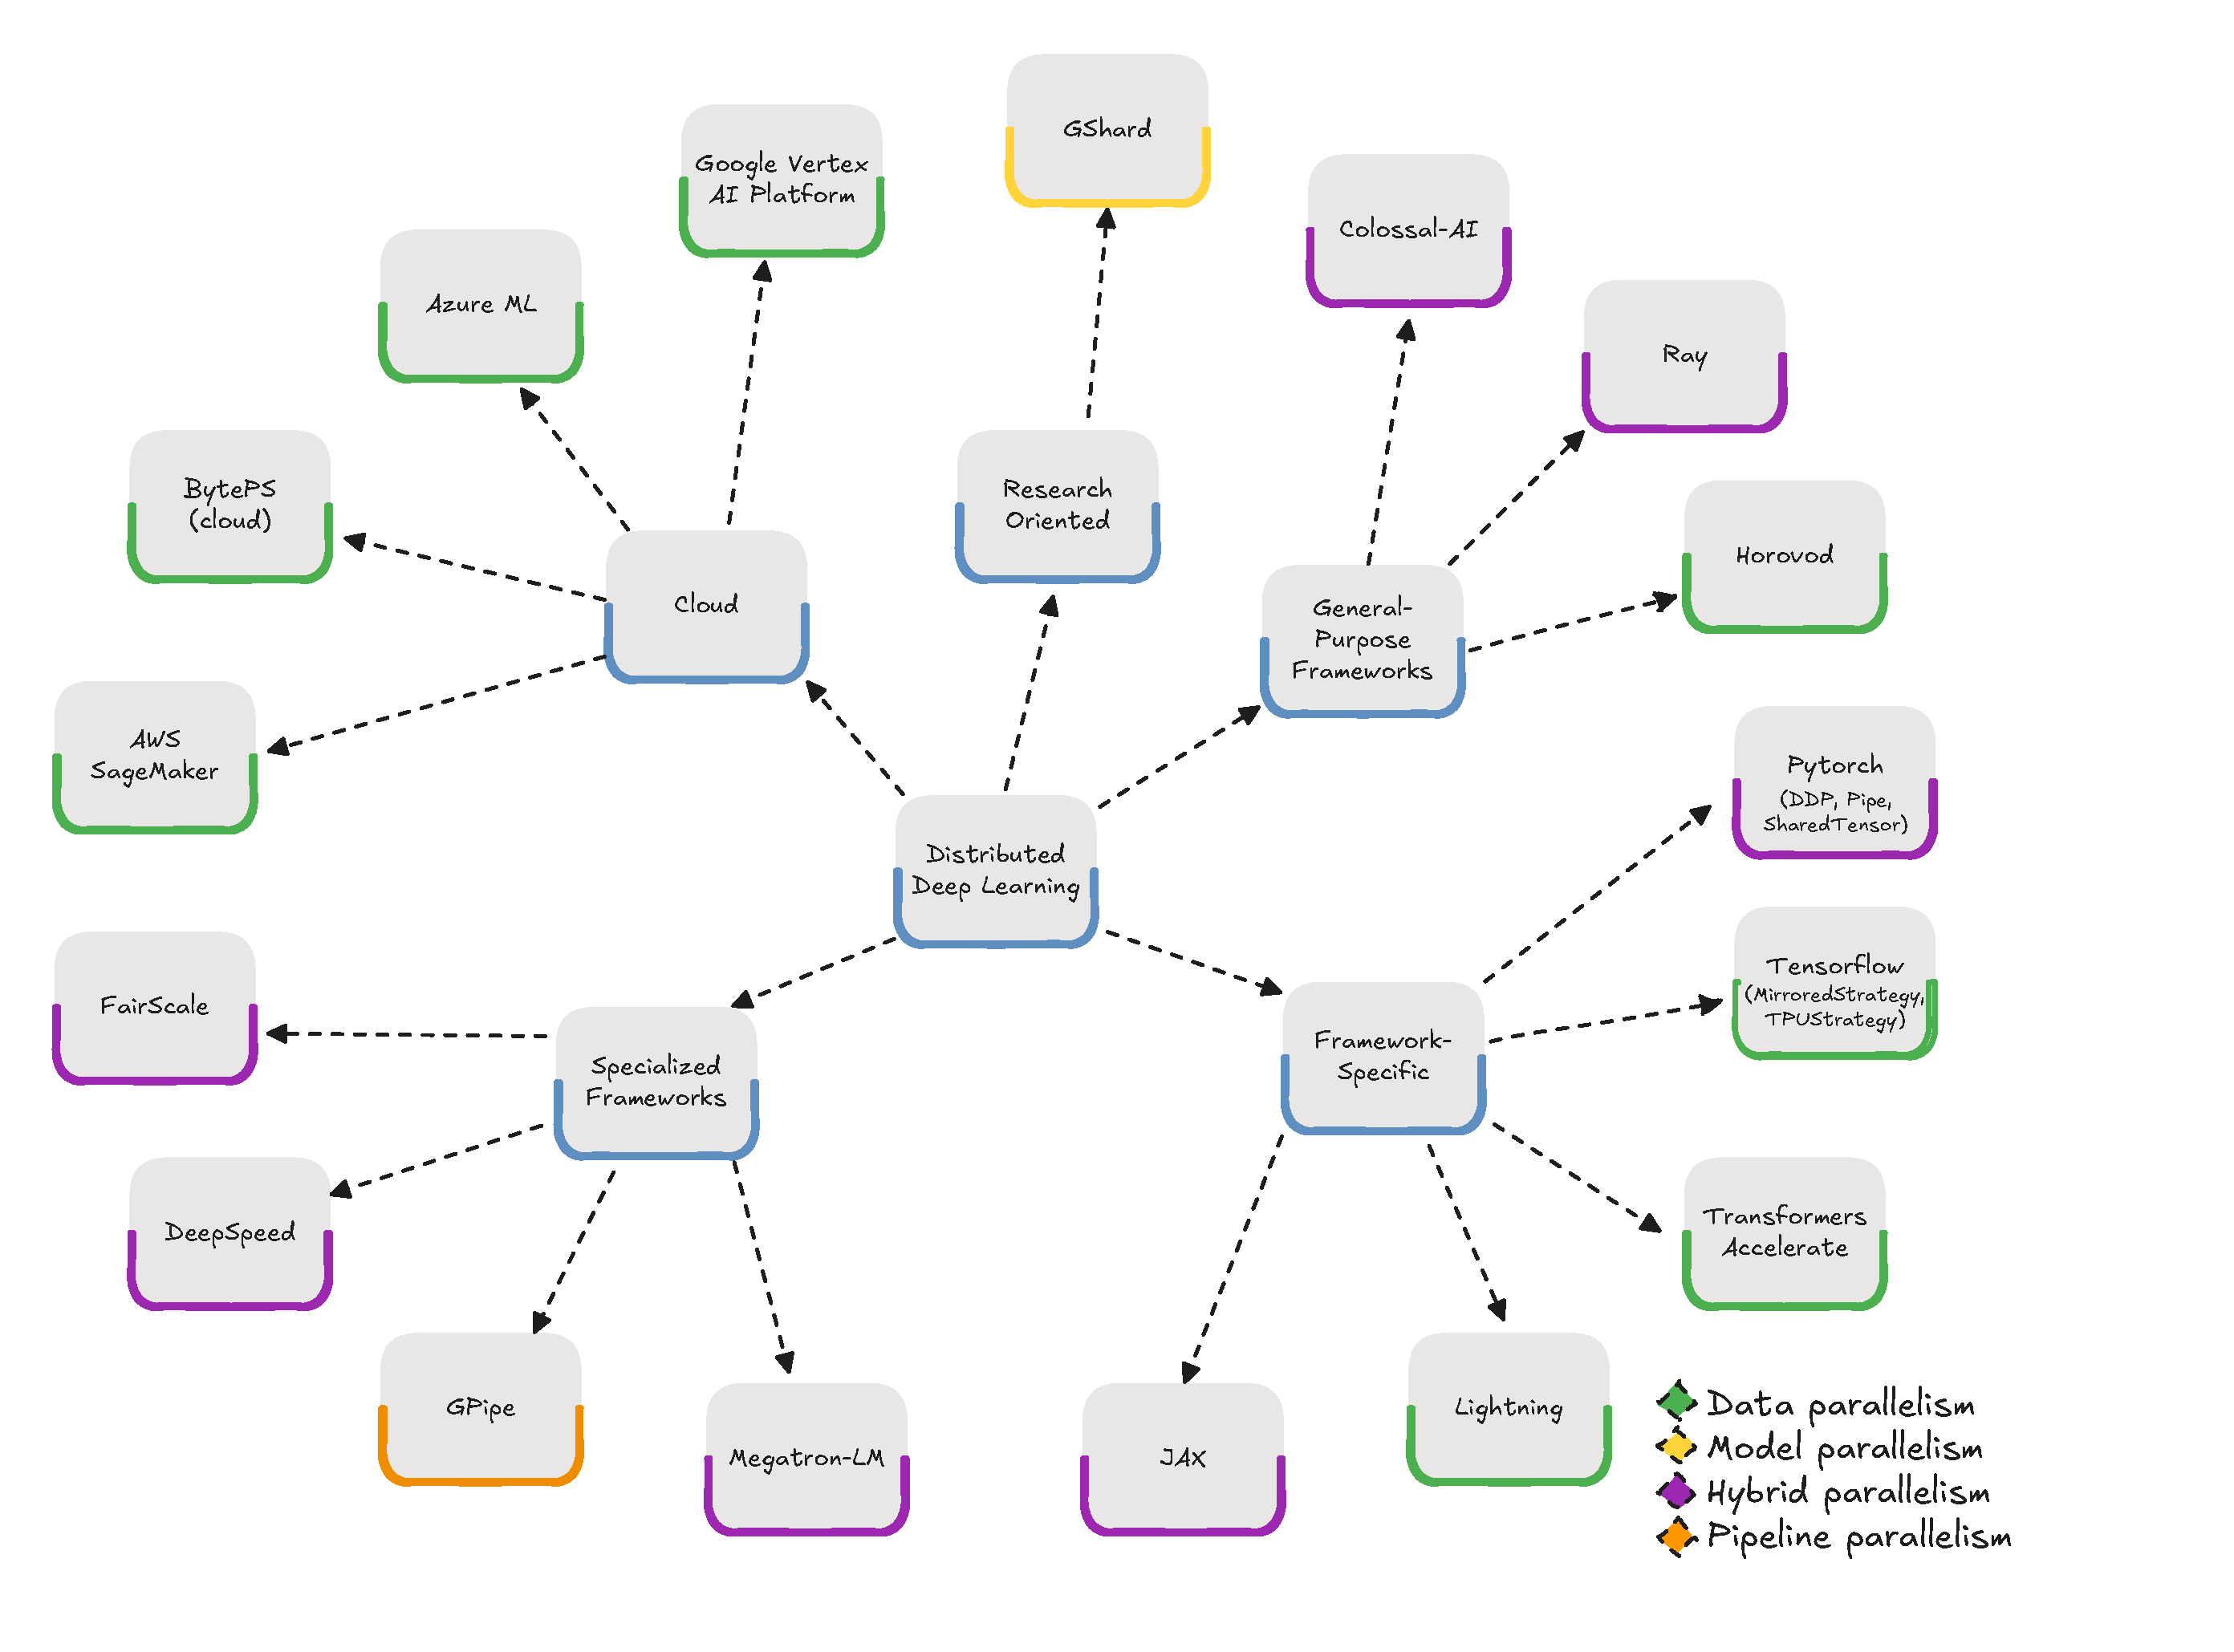
\includegraphics[width=\textwidth]{figures/mindmap}
		\caption{Accuracy for the EasyVQA training split.}
		\label{fig:base-a}
	\end{subfigure}
	\hfill
	\begin{subfigure}{0.48\linewidth}
		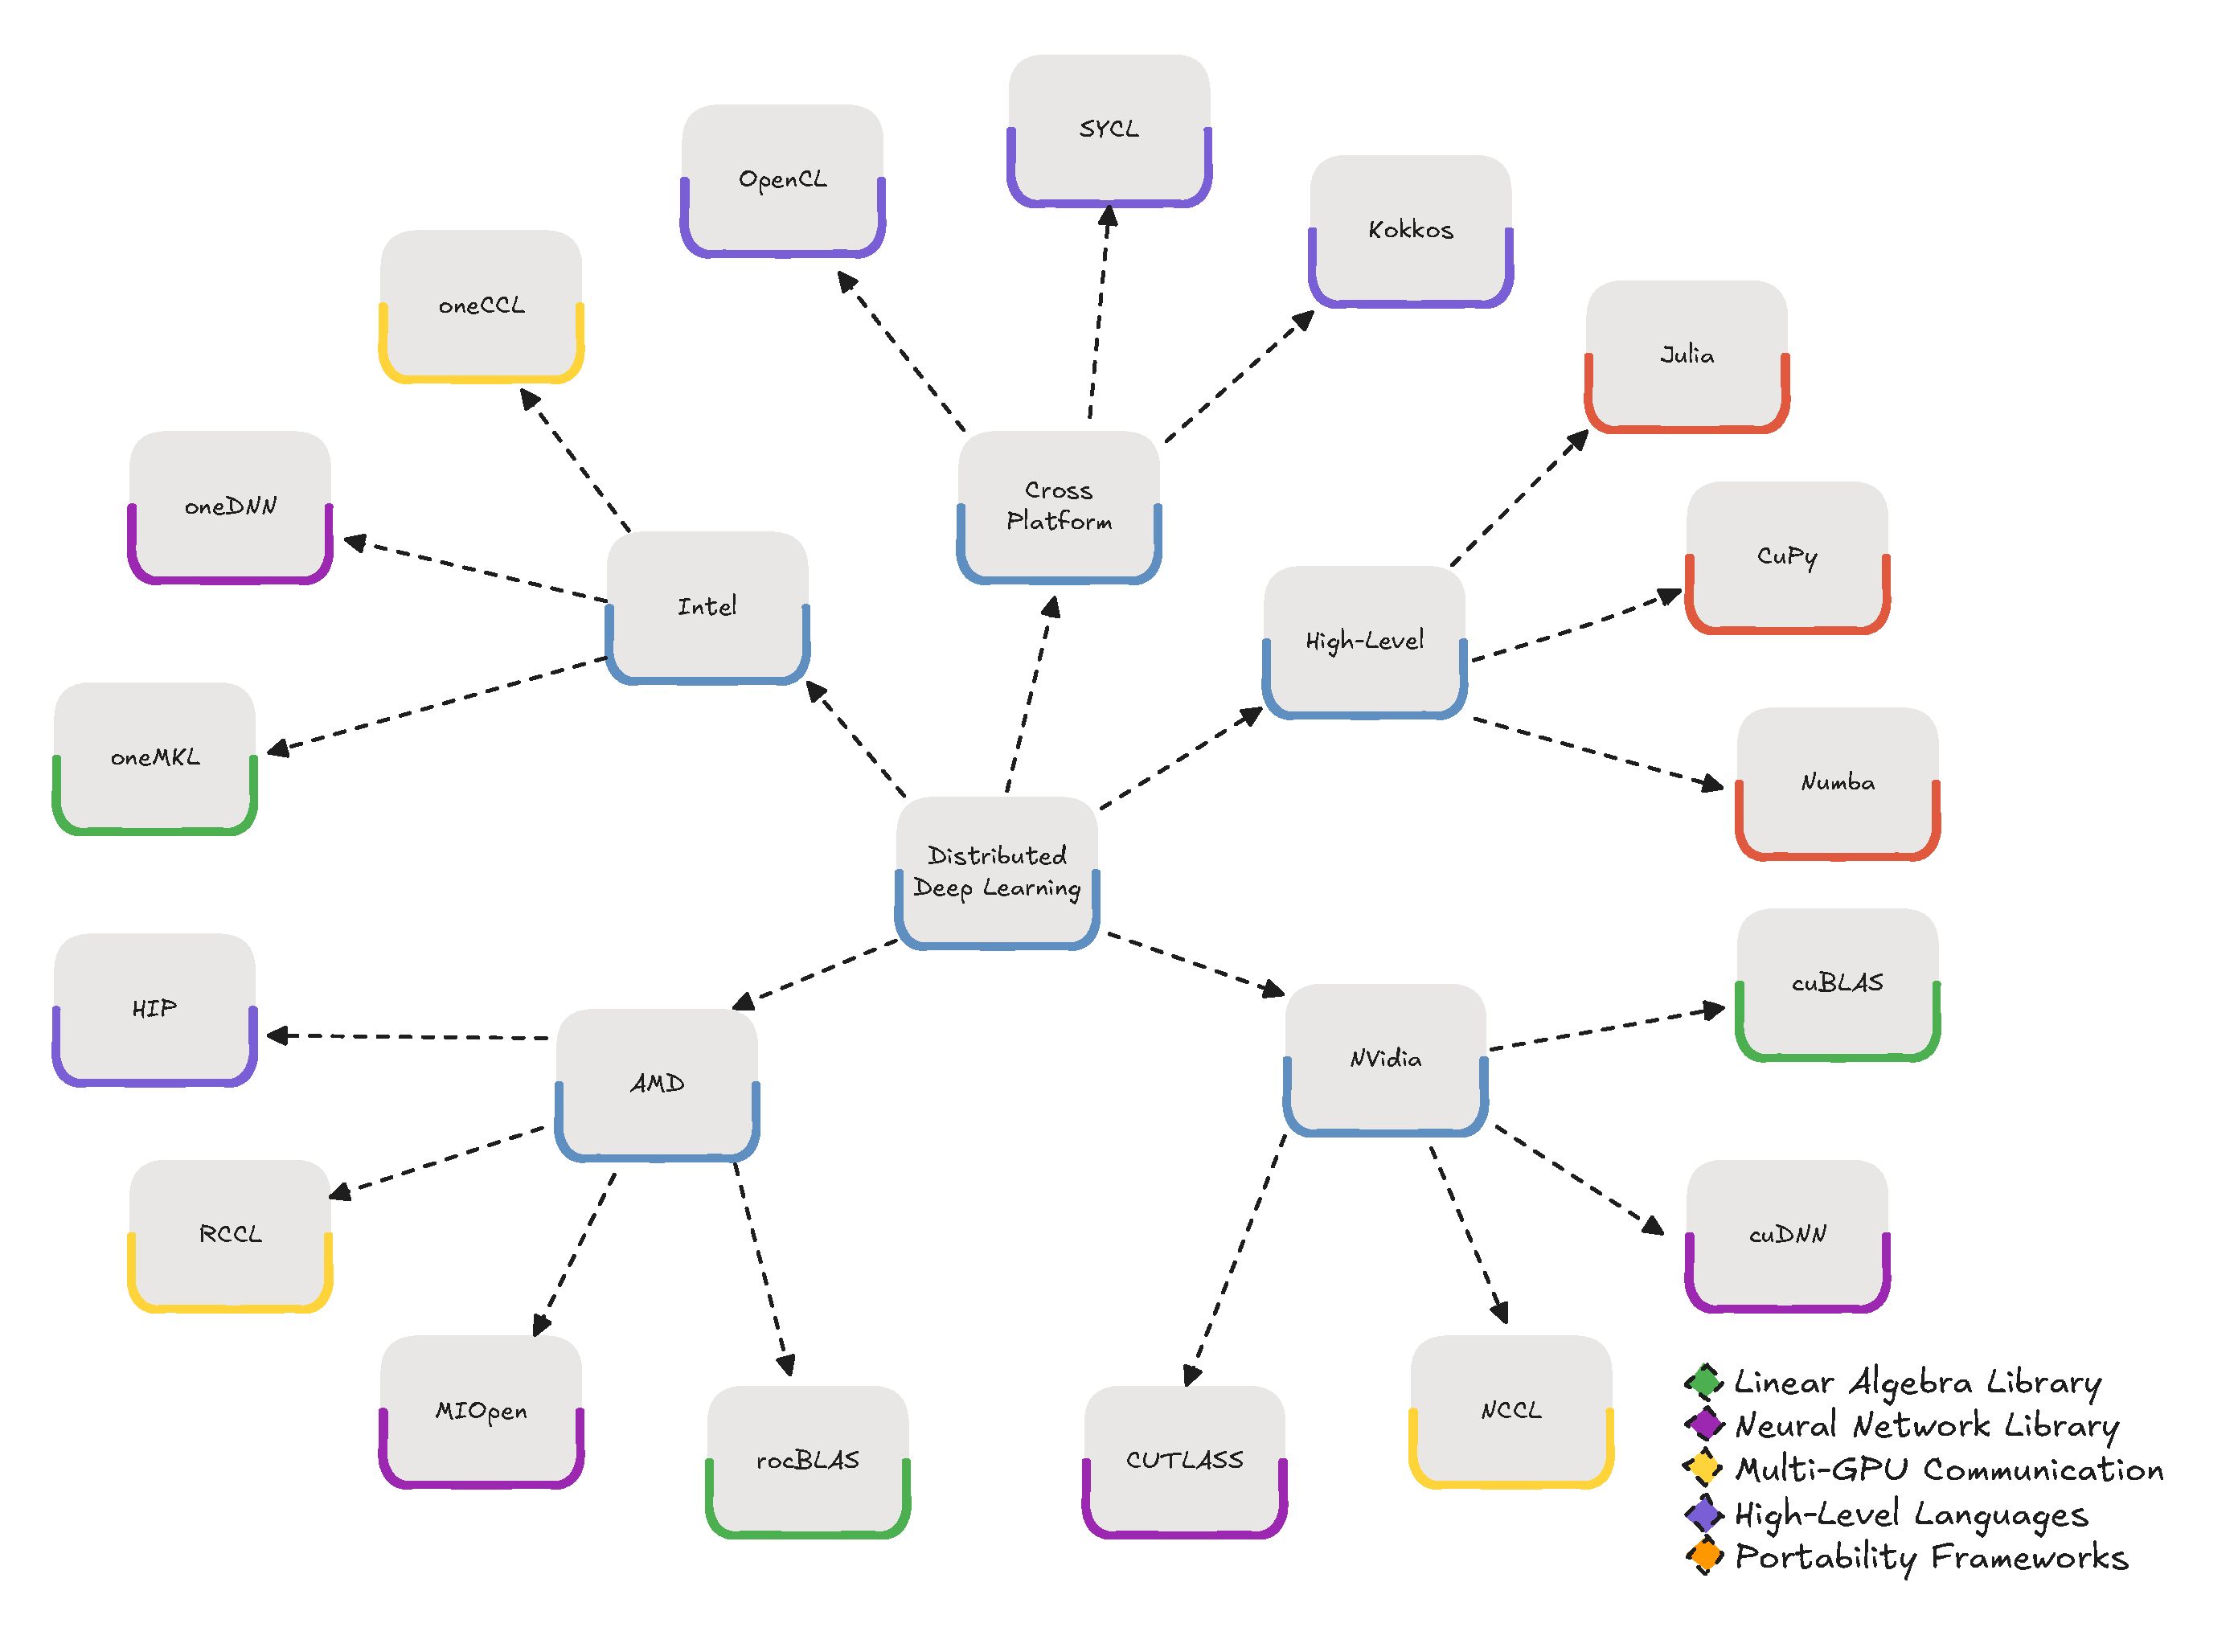
\includegraphics[width=\textwidth]{figures/mindmap-cuda}
		\caption{Accuracy for the DAQUAR training split.}
		\label{fig:base-b}
	\end{subfigure}
	\caption{Accuracy during training/validation on the baseline generator models.}
	\label{fig:base}
\end{figure*}

\begin{itemize}
	\item C1: Key Motivating Factors
	\item C2: Critical Factors and Guidelines
	\item C3: Practical Evaluation Scenarios
	\item C4: Tool Limitations and challenges
\end{itemize}

The resulting artifacts are available in the supplementary material in Table
\ref{tab:dnn_passages}. Each contributing factor is associated with an exact passage and various
codes (categories) that were used to classify the passage. The studies are summarized below.

\textbf{Motivating Factors.}
The motivating factors for training DNNs include the pursuit of better performance through more
efficient training and increased usability in practical scenarios. It has been widely regarded that
by scaling the architectures to a large number of parameters and leveraging larger datasets, the
evaluation accuracy on many benchmarks would be improved \cite{hestness_deep_2017}. However, it was
recently demonstrated by Deepseek R1
\cite{deepseekai2025deepseekr1incentivizingreasoningcapability} that scaling up the computational
power is not the only possible method of progress. As a result, future research is likely to focus
not only on distributed training, but also on innovating existing architectures.

Nonetheless, optimizing speed is crucial because by training larger models, performance is likely to
improve \cellrefs{D103} and as a result many applications become viable \cellrefs{D105}, which
otherwise would be infeasible to train.

It has been shown through empirical evidence that increasing the size of the model or dataset,
leads to better performance \cellrefs{D102,D105,D111}. This has been applied in industrial settings
\cellrefs{D101,D106}, and large scale training requirements have been formalized in
\cellrefs{D109,D110}.

Apart from scalability, performance is also a key motivating factor \cellrefs{D103,D105}. Some
studies have shown that increasing the depth of the network overcomes performance bottlenecks
\cellrefs{D103}, ensuring applicability in a wide range of domains. Lastly, resource utilization
also plays an important role in practical scenarios where clusters typically contain heterogeneous
hardware \cellrefs{D104}.

Beyond performance and scale, ease of programming and accessability to a wide range of uses also
play a crucial role. This involves simplifying workflows and enabling access to advanced techniques
to a wider audience \cellrefs{D110,D111,D112}. Nonetheless, one obstacle for usability is the
requirement to evolve existing frameworks and support an increasing number of applications as user
requirements change \cellrefs{D106}. Furthermore, cross-platform and cross-framework support remain
crucial for wider adoption and flexibility \cellrefs{D109,D112}, while at the same time enforcing
innovation through scientific curiosity \cellrefs{D102}.

\textbf{Critical Factors.}
There were considered several critical factors to effectively develop large machine learning systems.
Performance and scalability are among the central concerns \cellrefs{D203,D206,D207,D209,D212}. These
can further be trimmed down to efficiency (not waste resources), speed and the ability to handle
a wide range of architectural choices in distributed environments.

Usability and ease of use are also increasingly considered important for broader adaption and
developer productivity, which includes intuitive programming paradigms and simplified workflows
\cellrefs{D202,D205,D209,D211,D212}.

There are also other factors such as cost and communication efficiency which were also considered
\cellrefs{D209}. Particularly, they have been shown to represent a bottleneck \cellrefs{D204,D210},
and thus are also crucial.

To facilitate all these factors, effective hardware utilization (using both the CPU and GPU) plays
an important role \cellrefs{D201}, as well as software engineering principles like separation of
concerns \cellrefs{D205}, further contribute to robust library design.

\textbf{Evaluation Scenarios.}
Generally, evaluation is done by assessing task performance metrics, which includes accuracy
across various tasks like image classification, vision or NLP \cellrefs{D303,D305,D306,D308,D311}.
Although the measurements regarding the speed, efficiency or resource utilization are important
\cellrefs{D306,D307,D308,D311}, scalability is a key metric that is largely used in the literature
\cellrefs{D306,D308,D311}. In particular, studies such as \cellrefs{D301} assess deployment
in real-world scenarios.

Lately, some algorithms have also focused on cross-framework evaluation to ensure broader
applicability \cellrefs{D304}.

\textbf{Limitations and Challenges.}
The main challenges faced by DNNs include communication overhead and resource under-utilization
\cellrefs{D401,D403,D404,D405,D407,D410}. The lack of standardized tools and frameworks lead
to difficulties regarding programming complexity and ease of use \cellrefs{D402,D403,D408}.

There exist high-level optimization challenges that prevent achieving peak performance, due to
different architectures and hardware configurations \cellrefs{D406,D411}. Moreover, there exist
also algorithmic limitations, tight coupling, and issues related to debugging code
\cellrefs{D405,D406,D408,D411}, which shows that there is still large room for improvement.

Finally, the need for manual tuning and best-configuration selection points towards the need to
create more user-friendly machine learning frameworks \cellrefs{D411}.

\subsubsection{GPU Programming.}
\paragraph{Motivating Factors.}
Below are summarized the motivating factors for the development of GPU programming libraries,
making use of the characteristics displayed in Table \ref{tab:gpu_passages}.

\textbf{Scalability and performance optimizations.}
The development of GPU programming libraries is primarily driven by the need to increase
performance \cellrefs{G1013,G1031,G1051}. This is most often done through focused % Also G1011,G1071
optimizations involving the learning kernels, which can be thought of as the ability to perform
large matrix multiplications quicker or alternatively reducing the need for auxiliary memory. These
improvements are intrinsically linked to scalability and the ability to develop larger and more
powerful architectures \cellrefs{G1011,G1012,G1071}. Optimizing speed implies faster training
on larger datasets, while reducing memory allows to increase the complexity of the network on
the same hardware.

\textbf{Compatibility.}
Another important concern is related to the integration and compatibility of GPU libraries with
existing frameworks \cellrefs{G1013,G1014,G1015,G1062}. This is particularly important as seamless
compatibility streamlines development and promotes wider adoption. As an example, Caffe \cite{Jia.EtAl_2014a}
particularly emphasizes how time-consuming developing optimized code for individual architectures is.
To combat this, frameworks such as CuDNN~\cite{chetlur_cudnn_2014} aim to provide optimized network
implementations for NVidia GPUs across multiple GPU architectures.

\textbf{Usability and programming experience.}
Another important factor involves the usability and programming experience \cellrefs{G1031,G1071},
as they emphasize the creation of tools accessible to a broader audience. This ensures that most
ML libraries can build fast neural network primitives, which in the end can satisfy an increasing
need for more complex applications \cellrefs{G1012,G1016,G1017,G1061}.

\paragraph{Critical factors.}
Performance remains as the key concern encompassing not only raw speed but also portability across
different hardware architectures \cellrefs{G2011,G2012,G2021}.

\textbf{Scalability.}
Scalability is equally important for handling increasingly complex models and datasets \cellrefs{G2011,G2041}.
One factor that greatly contributes to scalability is the ability to fully utilize the available resources
across heterogeneous hardware. This poses significant design constraints as it requires to integrate
both CPUs and GPUs simultaneously during training \cellrefs{G2021,G2041}.

Another important factor that influences scalability is to create modular code through the
separation of concerns as some libraries have highlighted \cellrefs{G2012,G2041}.

One aspect that plays a role in scalability is how efficient inter-GPU communication is in
multi-GPU setups \cellrefs{G2051}. As we shall see this is tightly linked to the choice of the
communication library and is a key concern for both GPU programming and DNN frameworks
\cite{noauthor_uxlfoundationoneccl_2025,noauthor_nvidianccl_2025,noauthor_rocmrccl_2025}.

\textbf{Usability.}
Moreover, broader adoption requires libraries that are easy to use, as this ensures developer productivity
\cellrefs{G2041}.

Also, usability is facilitated by the adoption of declarative programming styles and a focus on
high-level design which excluded boiler-plate code as much as possible \cellrefs{G2012,G2061}.

\paragraph{Evaluation.}
Both quantitative and qualitative studies are performed to assess the performance.

\textbf{Quantitative evaluation.}
Specifically, quantitative metrics assess solutions based on measured performance like convolution speed
and general throughput, frequently benchmarked against established methods \cellrefs{G3011,G3013}.
One approach to assess raw performance involves varying mini-batch sizes against popular neural network
architectures \cellrefs{G3011}. This is related also to portability as it allows to reach top
performance without imposing constraints on architecture choices or the hyperparameters used
\cellrefs{G3012,G3013,G3061}. This is a metric to assess generalization capabilities.

\textbf{Generalization capabilities.}
Given that generalization is important, the documents also touch on the effectiveness of the neural
networks in different domains (i.e. reinforcement learning, computer vision, NLP, etc.), which
ensures broad applicability~\cellrefs{G3012,G3061}.

To ensure fair assessment, the libraries are often evaluated in deployed environments and serve
practical real world applications~\cellrefs{G3041}.

\textbf{Qualitative evaluation.}
These methods are used to assess subjective aspects like the visual quality of the results, as it was
seen in AlexNet~\cellrefs{G3051}. Lastly, it is crucial to keep in mind the context of the evaluation,
as they are usually tailored to specific model architectures and application areas. As a result,
there is always a certain degree of subjectivity involved in the assessment~\cellrefs{G3031}.

\paragraph{Limitations and Challenges.}
Despite progress, GPU programming faces multiple challenges, which arguably can be attributed to
the lack of a large open-source ecosystem and the use of closed-source proprietary hardware.

\textbf{Developer effort.}
One significant concern is that the kernel optimizations are time-consuming and require specialized
expertise about the dedicated GPU architecture \cellrefs{G4012,G4041}. Also, unless using standardized
libraries (i.e. cuDNN~\cite{chetlur_cudnn_2014}), the replication of results can be challenging as
execution times can vary significantly \cellrefs{G4041}.

\textbf{Performance bottlenecks.}
Performance bottlenecks are due to small matrix operations, which are generally inefficient \cellrefs{G4051,G4061},
but also due to communication overhead in cross-GPU communication \cellrefs{G4051}.

Algorithmic and memory constraints are also present, with some algorithms being limited by high
memory usage \cellrefs{G4013}, and others requiring specialized implementations for various corner
cases \cellrefs{G4013}.

\textbf{Evolving architectures.}
The field also faces ongoing challenges with evolving architectures, which involves both hardware advancements
but also new neural network innovations, requiring continuous adaptation~\cellrefs{G4011}.

\subsection{Determining the relationship between concepts}

\paragraph{Motivating factors.}\
Below I analyze the relationships between the two topics, while leveraging rows MF1-MF7 from Table
\ref{tab:translations_motivating_factors}.

\textbf{MF1. Scalability.}
The connection is that scalability is a major shared motivating factor for both DNNs and GPU programming.
The increasing scale of data and complexity of DNNs necessitates scalable solutions. GPU programming is
motivated by providing the tools and optimizations needed to achieve this scalability, enabling DNNs to
handle larger workloads, improve productivity, and become more cost-effective.

\textbf{MF2. Complexity and performance.}
The key shared motivator is to manage computational complexity while at the same time ensure higher accuracy
in common applications (i.e. NLP tasks). The increased accuracy is due to the guarantee that performance
is likely to increase thanks to the scaling laws that neural networks exhibit.
GPU programming directly provides the necessary primitives to facilitate the scaling laws and DNNs build on top of them.

\textbf{MF3. Critical in many domains.}
GPU programming itself might be considered a more specialized domain, but its motivation is connected to the
critical applicability of DNNs across many fields. GPU programming enable DNNs to function efficiently in
these domains by providing the building blocks. In this case, NVidia provides the optimized libraries, as
they know the hardware better than the general community.

\textbf{MF4. Heterogeneous hardware.}
While DNNs are motivated to use heterogenous hardware to ensure broader applicability and performance, GPU programming
acknowledge its importance by providing C APIs for CPU-GPU communication. Nonetheless, there do exist limitations
due to latency and sub-optimal bandwidth utilization in both domains. A related concern is that GPU libraries like cuDNN do not provide
integrated support for multi-GPU training, which must be achieved manually by the user. As a result there exist areas
for improvement in both domains.

\textbf{MF5. Applications.}
A shared motivation is to simplify development and improve the practical utility of both DNNs and GPU programming.
Both fields are driven by the need to make life easier for developers to leverage parallel hardware effectively,
and the motivation to fulfill practical requirements of simplified deployment and reproducible research.

\textbf{MF6. Leveraging existing tools.}
DNN development benefits from open-source frameworks, ensuring community-driven innovation. Conversely, GPU programming,
while often proprietary, builds on-top of other low-level libraries like cuBLAS. This shows a reliance on other
proprietary software, which although ensures high-performance, can arguably hinder innovation in the long term.

\textbf{MF7. Cross-framework use.}
Open-source DNN framework aim for cross-framework compatibility and usability to foster community innovation.
GPU programming libraries show a trade-off between low-level, highly optimized primitives (like cuDNN), and offering
user-friendly interfaces (like CuPy and Torch7). Code sharing is important in both areas, however there is limited
scope for GPU programming due to proprietary software.

\paragraph{Critical factors.}
Below I analyze rows CF1-CF7 from Table \ref{tab:translations_critical_factors}.

\textbf{CF1. Paradigms, programming ease.}
DNNs are generally flexible and often use popular interpreted programming languages like Python to facilitate
ease of use.
On the other hand, GPU programming usually relies on C++ and CUDA, which are critical in areas
where speed is a key concern. There has been broad concern about programming ease in GPU programming
as well, as there have slowly been built new frameworks that provide bindings to the dominant paradigms
(Python). This ensures a lowering entry barrier to GPU programming for DNN practitioners who are
often more familiar with Python.

\textbf{CF2. Scalability.}
Both domains address scalability by implementing a modular programming style. DNN frameworks abstract away
the distributed infrastructure complexity (by being able to easily select distributed strategies), while
GPU programming abstract away low-level hardware details, allow developers to focus on the application logic.

\textbf{CF3. Performance.}
Performance is a key concern for both DNNs and GPU programming. DNNs are
motivated by the need to minimize network bandwidth latency and achieve better scalability (as larger
models would likely achieve better performance), while GPU programming provides optimized deep-learning
primitives by optimizing large-matrix operations. To facilitate this, thorough knowledge of the GPU
architecture is required.

\clearpage
\onecolumn

{\footnotesize
	\begin{longtable}{|l|p{5cm}|p{5cm}|p{5cm}|}
		\caption{Translations of the motivating factors}\label{tab:translations}   \\

		\toprule
		ID & Distributed Neural Networks & GPU Programming & Translation \\
		\midrule
		\endfirsthead

		\multicolumn{4}{c}{Table \thetable{} -- continued from previous page}           \\
		\toprule
		ID & Distributed Neural Networks & GPU Programming & Translation \\
		\midrule
		\endhead
		\midrule
		MF1
		   & \textbullet\ Google internally requires their deep learning frameworks to be scalable. \cellref{D101} \newline
             \textbullet\ Internally, other organizations (i.e. Facebook) become more and more reliant on neural networks. \cellref{D106}
           & \textbullet\ Optimizing kernels is difficult and time-consuming. \cellref{G1011}              
           & \uline{\textbf{Scalability}}\newline 
           %Internal need for scalability
           There is a surging \textbf{need for scalability}, likely due to the increasingly abundant \textbf{data availability} which time consuming to process. 
             The resulting reliance of neural networks has \textbf{increased productivity} and \textbf{reduced costs}.            \\
           \midrule
		   MF2 
           & \textbullet\ The trend to scale up datasets/computational resources is successful in competitions like ImageNet. \cellref{D102}, \cellref{D105}, \cellref{D103}
            \newline
            \textbullet\ The abundance of computation and data are particularly effective in Natural Language Processing (NLP) tasks. \cellref{D111}
           & \textbullet\ Natural parallelizability of deep learning techniques enables training higher capacity networks on larger datasets. \cellref{G1012} \newline
             \textbullet\ Early open-source GPU implementations of CNNs set precedent for code sharing. \cellref{G1051}
           & \uline{\textbf{Complexity and performance}}\newline 
           The GPU programming field enabled DNNs through \textbf{easy parallelization} of training. Larger networks consistently provide better \textbf{performance}, leading to widespread adoption, especially in \textbf{NLP tasks}. Open-source implementations have accelerated progress. \\
           \midrule
		   MF3 
           &
             \textbullet\ The deep learning applications are critical in many domains. \cellref{D103}, \cellref{D105} \newline
             \textbullet\ Frameworks have been extended reinforcement learning \cellref{D208}

           & \textbullet\ Deep learning frameworks (Caffe and PADDLE) rely on GPU programming libraries such as cuDNN. \cellref{G1014} \newline
             \textbullet\ As architectures evolve, underlying code needs to be re-optimized. This is standardized by NVidia as they understand better how the GPU architecture works.\cellref{G1013}
           & \uline{\textbf{Critical in many domains}}\newline 
           \textbullet\ GPU programming libraries are used in a more narrow domain, however DNNs have broader applicability in areas such as reinforcement learning. 
           \newline
           \textbullet\ NVidia understands well the GPU architecture and can provide better optimizations in critical areas.\\

           \midrule
		   MF4 
           & \textbullet\ Data centers are inherently homogenous. BytePS can leverage spare CPU and bandwidth resources to accelerate distributed training running on GPUs. \cellref{D104} \newline
             \textbullet\ Modern systems can leverage mobile devices, tablets, and thousands of GPU cards. \cellref{D201}
           & GPU programming libraries expose a C language API to communicate with the host CPU. \cellref{G1015}
           & \uline{\textbf{Heterogenous hardware}}\newline 
           There is limited support for CPU-GPU interaction in GPU programming libraries. However, heterogeneous hardware plays a more important role in DNNs as the ability to fully utilize available resources is critical. \\
 
           \midrule
		   MF5
           & DDNs have powered a wide range of applications including image recognition, language translation, anomaly detection, and more. \cellref{D106} \newline
             \textbullet\ Replication of published results can involve months of work by researchers. \cellref{G1041}
           & GPU libraries meet user's needs by reducing the need to write custom code, allowing developers to focus on higher-level issues, improved portability. \cellref{G1016} \newline
             \textbullet\ Few toolboxes offer truly off-the-shelf deployment of state-of-the-art models that are computationally efficient. \cellref{G1041}
           & \uline{\textbf{Requirements and applications}}\newline 
           Both topics aim to make it easier for developers to take advantage of parallel hardware. GPU programming facilitates the development of new architectures and DNNs scale models to achieve better accuracy. The need for efficient deployment and replication of research results drives development in both areas. \\

           \midrule
		   MF6
           & Colossal-AI builds on existing open-source frameworks such as PipeDream, GPipe and Chimera. \cellref{D107}, \cellref{D207}
           & \textbullet\ CuDNN relies on the CUDA toolkit, specifically the cuBLAS library. \cellref{G1016} \newline \textbullet\ CuPy is specifically designed to work with NVidia GPUs. \cellref{G1062}
           & \uline{\textbf{Leverage existing frameworks}}\newline 
           Since DNN frameworks are generally open-source, this encourages community involvement, which leads to innovation. \newline 
           GPU programming libraries are proprietary. Nonetheless, internally libraries such as cuDNN rely on the CUDA toolkit. \\

           \midrule
		   MF7
           & \textbullet\ Inter-GPU communication frameworks require minimal code changes and support multiple frontends. \cellref{D110}, \cellref{D112} \newline
            \textbullet\ Libraries can generally be integrated into existing frontend frameworks (i.e. PyTorch). \cellref{D211}
           & \textbullet\ GPU programming libraries provide lower-level primitives and are generally self-contained. \cellref{G1017} \newline
             \textbullet\ Libraries emphasize compatibility (CuPy with NumPy) or ease of development (Torch7). \cellref{G1062}, \cellref{G1071} \newline
             \textbullet\ Research-focused libraries prioritize configurability and flexibility. \cellref{G1031}
           & \uline{\textbf{Cross-framework use}}\newline 
           Open-source DNN libraries promote usability and cross-framework compatibility, fostering innovation. GPU libraries vary between low-level primitives (cuDNN) and user-friendly interfaces (CuPy, Torch7), though being closed-source limits community-driven innovation. This highlights the importance of code sharing for research. \\

           % recent advancements in deep learning
           % rapidly evolving field

        

		\bottomrule
	\end{longtable}
}

\twocolumn

% DONE D101 internal need for scalability
% DONE D102 increasingly complex datasets (Done also from D105 and D111), Improved performance
% DONE D103 critical in many domains (emerging applications)
% DOING D104 utilization of heterogeneous hardware
% D105
% howpublished = \{(https?://.*?)\}
% howpublished = {\url{$1}}
% url = \{(https?://.*?)\}
% howpublished = {\url{$1}}
% DONE D201 utilization of heterogenous hardware


% Not taken into account:
% D108
\clearpage
\onecolumn

{\footnotesize
	\begin{longtable}{|l|p{5cm}|p{5cm}|p{5cm}|}
		\caption{Translations of the critical factors}\label{tab:translations_critical_factors}   \\

		\toprule
		ID & Distributed Neural Networks & GPU Programming & Translation \\
		\midrule
		\endfirsthead

		\multicolumn{4}{c}{Table \thetable{} -- continued from previous page}           \\
		\toprule
		ID & Distributed Neural Networks & GPU Programming & Translation \\
		\midrule
		\endhead
		\midrule
		CF1
		   & Generally DNNs are most flexible and use the most common programming style supported by the host language. \cellref{D202}, \cellref{D205}
           & \textbullet\ Although most GPU frameworks work using the host language as C++, there exist frontend frameworks that enable users to use Python. \cellref{G2061} \newline
             \textbullet\ Cudnn exposes a C API \cellref{G1015} \newline
             \textbullet\ Torch7 is designed for ease of programming through Lua \cellref{G2021} \newline
             \textbullet\ CuPy implements NumPy-like API \cellref{G2061}
           & \uline{\textbf{Paradigms, programming ease.}}\newline
           Imperative and declarative programming styles are both supported. DNNs use Python as the most popular host language, while GPU frameworks generally work with C++ and CUDA. 
           Nonetheless, there do exist frontend frameworks that enable users to write code in higher-level languages (i.e. Lua, Python), and compatibility libraries (NumPy-like API) to improve accessability.\\
           \midrule

    CF2
    & \textbullet\ Distributing neural network layers across multiple GPUs is architecture-specific. \cellref{D203} \newline
      \textbullet\ Scaling is expensive in terms of cost, time and code integration. \cellref{D209} \newline
      \textbullet\ There is a separation of concerns between GPU programming and DNNs, as there is no need for custom C++ code or compiler required to distribute neural networks over cluster nodes. \cellref{D211}
        & \textbullet\ Optimized code using NVIDIA GPUs ensures high performance (freeing up auxiliary memory) \cellref{G2011} \newline
          \textbullet\ CuDNN provides separation of concerns by enabling developers to focus on higher-level optimizations instead of low-level architecture specific code \cellref{G2012} \newline
          \textbullet\ Caffe implements separation of representation and implementation \cellref{G2041}
        & \uline{\textbf{Scalability, separation of concerns.}}\newline
        \textbullet\ Scalability challenges are related to distributing parts of the network or dataset across multiple nodes. Frameworks emphasize separation of concerns, allowing developers to focus on higher-level optimizations while library providers handle hardware-specific optimizations.\\
        \midrule

    CF3
    & \textbullet\ Specialized techniques for distributed training include: bucketing, overlapping communication with computation, etc. \cellref{D206} \newline
      \textbullet\ Megatron-LM extends optimization techniques to the transformer model. \cellref{D211}
        & \textbullet\ Libraries optimize for wide range of use cases \cellref{G2011} \newline
          \textbullet\ Frameworks like Torch7 leverage SSE and support multiple parallelization methods \cellref{G2021}
        & \uline{\textbf{Performance optimization.}}\newline
        Both domains focus heavily on performance optimization through various techniques. DNNs use specialized distributed training techniques, while GPU frameworks optimize for different architectures and use cases through various parallelization methods.\\
        \midrule
    
    CF4
    & There exist algorithms that can optimize network latency. \cellref{D210} \cellref{D204}
        & \textbullet\ Multi-GPU training is an outstanding challenge \cellref{G4011} \newline
          \textbullet\ GPUs can read/write directly to each other's memory \cellref{G2051} \newline
          \textbullet\ Inter-GPU communication is optimized for specific layers \cellref{G2051}
        & \uline{\textbf{Network and hardware communication.}}\newline
        While optimal algorithms exist for network latency optimization, multi-GPU training presents ongoing challenges. AlexNet optimized inter-GPU communication through direct memory access and selective layer communication. The CuDNN leaves multi-GPU communication to the user.\\
        \midrule

    CF5
    & The Transformers library provides modular components that greatly simplify the extension and ease of use of the library \cellref{D212}
        & \textbullet\ CuPy is NumPy compatible \cellref{G1062} \newline
          \textbullet\ CuDNN requires more specialized C and CUDA knowledge \cellref{G1015} \newline
          \textbullet\ Caffe provides easy CPU/GPU switching and clean Python/MATLAB bindings \cellref{G2041}
        & \uline{\textbf{Ease of use and hardware flexibility.}}\newline
          \textbullet\ DNN libraries emphasize modularity and ease of extension. \newline
          \textbullet\ GPU frameworks vary in accessibility - some require specialized knowledge while others provide familiar APIs and easy hardware switching capabilities.\\
        \midrule

		\bottomrule
	\end{longtable}
}

\twocolumn


\clearpage
\onecolumn

{\footnotesize
	\begin{longtable}{|l|p{5cm}|p{5cm}|p{5cm}|}
		\caption{Translations of the evaluation metrics}\label{tab:translations_evaluation_metrics}   \\

		\toprule
		\textbf{ID} & \textbf{Distributed Neural Networks} & \textbf{GPU Programming} & \textbf{Translation} \\
		\midrule
		\endfirsthead

		\multicolumn{4}{c}{Table \thetable{} -- continued from previous page}           \\
		\toprule
		\textbf{ID} & \textbf{Distributed Neural Networks} & \textbf{GPU Programming} & \textbf{Translation} \\
		\midrule
		\endhead
		\midrule
    EM1
        & \textbullet\ Evaluation was initially performed behind closed doors for internal processes (speech recognition systems) and subsequently for external applications (Google Search). \cellref{D301}
        & \textbullet\ In many frameworks, the GPU libraries can be switched on and off at compile time using a single flag. \cellref{G1014} \newline
          \textbullet\ Some are designed for both research and industry, run on both CPU and GPU, have bindings for both Python and Matlab. For model architecture portability, Protocol Buffer files are used. \cellref{G3041}
        & \uline{\textbf{Deployment:}} \newline
          \textbullet\ Large companies employ staged deployment: first testing internally before external applications, enabling safe evaluation. \newline
          \textbullet\ Framework designers can rollback through compile-time flags. CUDA code written in C, with Python and Matlab bindings ensure portability.
        \\
        \midrule

    EM2
        & \textbullet\ The evaluation was done by scaling complex networks -- based on Mixture of Experts -- to 600B parameters using automatic sharding. \cellref{D305}
        & \textbullet\ The cuDNN library is assessed by measuring time and memory usage for convolutional layers. 
        Mini-batch performance is also assessed.
        Scalability is not as much of a concern as different GPU architectures are benchmarked instead of assessing performance across GPU clusters. \cellref{G3011}
        & \uline{\textbf{Model Architectures:}} \newline
          \textbullet\ Scalability testing is a concern for DNNs, as these are the type of problems that are encountered in the real world. \newline
          \textbullet\ However, for GPU programming, performance is measured by optimizing resource usage on a single GPU. 
          The difficulty stands in optimizing performance as new NN architectures are developed.
        \\
        \midrule

    EM3
        & \textbullet\ Evaluation tasks include: image classification \cellref{D303}, machine translation \cellref{D303}, \cellref{D305}, 
          NLP \cellref{D306} \cellref{D311}, RL \cellref{D308}.\newline
          \textbullet\ MoE models can be scaled up to 600 billion parameters for machine translation.
        & \textbullet\ CuDNN can be used in deep learning, CNNs, speech and language. \cellref{G3012} \newline
          \textbullet\ CuPy can be extended to scientific computing and probabilistic modelling. \cellref{G3061}
        & \uline{\textbf{Task Domains:}} \newline
          \textbullet\ DNN libraries focus on deep learning tasks. \newline
          \textbullet\ CuDNN was designed for deep learning. CuPy can be used in broader domains.
        \\
        \midrule

    EM4
        & \textbullet\ Impressive improvements in performance over older methods. \cellref{D304} \newline
          \textbullet\ Evaluation is done against vision and NLP tasks \cellref{D306} and RL \cellref{D308}. \newline
          \textbullet\ Wikipedia dataset is often used for evaluation. \cellref{D307} \newline
          \textbullet\ Scaling gives consistent improvements in performance. \cellref{D311}
        & \textbullet\ Evaluation metric involves assessing performance and matrix multiplication. Speedup reaches up to 36\% improvements. \cellref{G3013} \newline
          \textbullet\ CuDNN is assessed against libraries like cuda-convnet2 and Caffe. Achieves portability across GPU architectures. \cellref{G3013} \newline
          \textbullet\ Qualitative evaluation can offer valuable insights into performance. \cellref{G3051}
        & \uline{\textbf{Evaluation:}} \newline
          \textbullet\ Potential for gains through hardware-specific optimizations. \newline
          \textbullet\ Broad applicability of DNNs, while GPU programming focuses on specific architectures. \newline
          \textbullet\ Consistent scaling suggests promising future for DNNs, while GPU advances focus on specific implementations.
        \\
        \midrule

    LF1
      & \textbullet\ To address usability, many libraries provide common APIs with other frameworks. \cellref{D402} \newline
        \textbullet\ Training DNNs require special algorithms that are often architecture-specific. \cellref{D403} \newline
        \textbullet\ Optimizations are challenging and error prone, requirement intimate knowledge of the network architecture. \cellref{D411} \newline
        \textbullet\ Reinforcement learning libraries have bindings that allow both task-parallel and actor-based parallelism. \cellref{D408}
      & \textbullet\ Replication of results is challenging (can take months of work). \cellref{G4041} \newline
        \textbullet\ The requirement to manually fine-tune architectures is time-consuming and requires deep knowledge of the GPU architecture. \cellref{G4012} \newline
        \textbullet\ The memory profiles are used to assess performance. \cellref{G4012}
      & \uline{\textbf{Usability:}} \newline
      \textbullet\ To address the replication of SOTA results common APIs are used (Transformers~\cite{wolf_huggingfaces_2020} addresses this issue as it interfaces with \cite{falcon_pytorch_2019}). \newline
      \textbullet\ Being closed source, open-source frameworks cannot reliably match NVidia SOTA performance, as they have better knowledge of the GPU architecture. \newline
      \textbullet\ Profiles are key to efficient debugging and optimization in both cases.\\
      \midrule

    LF2
        & \textbullet\ No single algorithm that can perform optimally across all cases. \cellref{D406} \newline
          \textbullet\ Communication overhead leads to resource under-utilization and solutions do not transfer across architectures. \cellref{D403}, \cellref{D405} \newline
          \textbullet\ Data parallelism models are designed for homogeneous setups. \cellref{D404}
        & \textbullet\ Main issues relate to memory management around matrix multiplication algorithms. Problems also relate to hyperparameter choice, as some stride sizes perform sub-optimally. \cellref{G4013}
        & \uline{\textbf{Algorithmic Limitations:}} \newline
          \textbullet\ No algorithms perform optimally across all cases. \newline
          \textbullet\ Memory optimizations remain a challenge for both GPU programming and DNNs.
        \\
        \midrule
        
    LF3
        & \textbullet\ Tensorflow performs node placement and communication management which results in overhead. \cellref{D401} \newline
          \textbullet\ Deepspeed incurs communication overhead by allocating data to CPU memory. \cellref{D407} \newline
          \textbullet\ Some papers emphasize collaboration in the research community to ensure innovation. \cellref{D410}
        & \textbullet\ Sophisticated techniques to manage communication overhead by not updating parameters across GPUs on each layer. \cellref{G4051} \newline
          \textbullet\ The cost of transferring data to the GPU outweighs the benefits of using a GPU. \cellref{G4061} \newline
          \textbullet\ The very existence of CuDNN implies that cross-GPU programming is challenging which requires thorough understanding of the GPU architecture. \cellref{G4012}, \cellref{G4011}
        & \uline{\textbf{Communication Overhead \& Scalability:}} \newline
          \textbullet\ Tradeoffs between communication overhead and performance. \newline
          \textbullet\ Both GPUs and DNNs face similar bottlenecks in terms of memory allocation that impacts performance. \newline
          \textbullet\ There are no simple universal solutions and choosing the right approach depends on model architectures and hardware. \newline
          \textbullet\ Community is key to success for DNNs.
        \\
        \midrule


        
		\bottomrule
	\end{longtable}
}

\twocolumn



\textbf{CF4. Network and hardware communication.}
Multi-GPU training is particularly relevant in DNNs. There exist multiple algorithms to minimize
network latency, however GPU programming frameworks still struggle with multi-GPU communication
training, as libraries like cuDNN leave this management to the user. This indicates an ongoing challenge
in this area.

\textbf{CF5. Ease of use and hardware flexibility.}
The main challenge here resides between ease of use to the developer and hardware flexibility.
Considering the broad community of developers, DNN libraries prioritize modularity and ease of
extension to facilitate usability. Some GPU programming libraries sacrifice ease of use for lower-level control
and potentially higher performance (cuDNN), while others strive for more user-friendly API and easier
hardware switching (CuPy, Caffe).
\paragraph{Evaluation.}
Finally, these are the evaluation metrics (EM) for each domain, together with the challenges and
ongoing limiting factors (LF) for each domain.

\textbf{EM1. Deployment.}
Deployment is an important aspect for both DNNs and GPU programming. DNN libraries follow a staged
deployment process for safe evaluation (i.e. Google products), which offers a degree of safety in
real world scenarios. Conversely, GPU programming frameworks are designed with configurable deployment
in mind, providing features like compile-time flags to integrate more easily into ML frameworks.

\textbf{EM2. Model architectures.}
In some evaluating scenarios, special care was payed to assess performance across different architectures.
For DNNs, this involves assessing scalability with increasingly complex model architectures. On the other hand,
for GPU programming evaluation is geared towards optimizing performance by providing efficient primitives
for the most popular operations (convolutions, self-attention, fully connected layers, etc.).

\textbf{EM3. Task domains.}
Evaluation metrics are strongly dependent on the task domains. DNN benchmarks are performed across
a broad spectrum of deep learning tasks to show general applicability. GPU programming libraries,
while generally geared towards deep learning tasks (like cuDNN), some tools also aim for broader
use (like CuPy in scientific computing). As a result, GPU programming focuses on depth by ensuring
high-performance in a focused field, while DNNs aim for breadth by showing general applicability.

\textbf{EM4. Evaluation}
DNN evaluation focuses on overall performance gains and broad applicability in different domains (vision,
NLP, etc.). GPU programming, on the other hand, focuses on the potential performance gains achievable through
hardware-specific optimization. This shows that older approaches are continuously refined when new hardware
becomes available, which in turn affects the design of DNNs.

\textbf{LF1. Usability.}
Usability is a limitation factor that affects both areas, with repercussions around reproducibility and developer
productivity. DNN libraries attempt to improve usability through common APIs to facilitate broader
experiment reproducibility. On the other hand, although closed-source GPU programming frameworks
demonstrate better performance due to a more through understanding of the underlying hardware, this sacrifices
developer productivity. For example, debug information is often hidden to the user to avoid leaking
internal implementation details. This is often combated through the use of complex workflows using
profiling tools.

\textbf{LF2. Algorithmic limitations.}
The primary algorithmic limitation concerns memory management in both domains.
DNNs pose problems related to data and model parallelism, while GPU programming faces issues
related to matrix multiplication algorithms and hyperparameter choices being suboptimal in some edge cases
(i.e. small batch size). This shows that advancements are needed in both areas.

\textbf{LF3. Communication Overhead and Scalability.}
Another limitation is the communication overhead and its impact on scalability. Both areas struggle
with this, leading to performance bottlenecks that are challenging to overcome. There are not universally
optimal solutions, as the best approaches are dependent on model architectures and hardware configurations.
Community involvement is essential for progress as this has proven to promote innovation and faster progress.

\subsection{Study Selection Results}
\label{sec:study_selection_results}
The complete lists of included and excluded studies, along with detailed information about each study, can be found in the supplementary materials (Section \ref{sec:study_selection}). A total of XXX studies were initially identified, with XXX studies meeting our inclusion criteria after screening. Table \ref{tab:study_types} provides an overview of the types of studies included in our review.

% \begin{table*}[ht]
% 	\centering
% 	\caption{Overview of Included Study Types}
% 	\label{tab:study_types}
% 	\begin{tabular}{|l|c|p{8cm}|}
% 		\hline
% 		\textbf{Study Type}    & \textbf{Count} & \textbf{Description}                                                     \\
% 		\hline
% 		Empirical Studies      & XXX            & Studies with experimental evaluations of distributed learning techniques \\
% 		\hline
% 		Implementation Studies & XXX            & Studies focusing on CUDA implementations and optimizations               \\
% 		\hline
% 		Hybrid Studies         & XXX            & Studies covering both theoretical and implementation aspects             \\
% 		\hline
% 		\textbf{Total}         & XXX            &                                                                          \\
% 		\hline
% 	\end{tabular}
% \end{table*}

\begin{itemize}
	\item \textbf{Goals:}
	\item To analyze parallelization frameworks in DDL.
	\item To evaluate libraries that support CUDA programming.
	\item To find out how these concepts are intertwined.
	\item To get practical experience with popular frameworks. \\
	\item \textbf{Expected Outputs:}
	\item Experience for conducting a systematic review.
	\item Systematic mapping of programming frameworks.
	\item Comparative analysis with strengths and weaknesses.
	\item Identification of research gaps. \\
	\item \textbf{Constraints:}
	\item Time period limited to 2012-2024\footnote{CUDA: 2012 is the year when AlexNet was published.} and
	      2015-2024\footnote{DDL: 2015 is the year when the shift towards scalability was noticed.}.
	\item Peer-reviewed articles and conference papers only.
	\item English language publications only.
	\item Technical implementation details must be present. \\
	\item \textbf{Search Terms and Keywords:}
	\item Listed in Table \ref{tab:search_terms}.
\end{itemize}

